\part{Développer une application en Python pour évaluer les modèles HTR}\label{partie_3}

La deuxième partie du stage était axée sur une mission de développement applicatif. 

Au sein d'ALMAnaCH, il s'agissait de disposer d'un outil interne permettant de visualiser rapidement des informations sur la qualité des transcriptions réalisées par les modèles HTR entraînés avec le CLI \textit{Kraken}. 

Cependant, l'outil devait être généralisable, pour être réutilisé dans d'autres projets. Il était souhaitable, également, que l'application prenne en ligne de compte la possibilité, à terme, d'interagir avec le fichier XML-TEI pivot pour importer les transcriptions HTR et les vérités terrains d'\textit{eScriptorium} et récupérer les métriques d'évaluation. 

L'application \textit{Kraken-Benchmark}, créée durant mon stage, a permis de réaliser en partie ces objectifs.\footnote{La seconde mission de stage a été présentée sous la forme d'une \textit{issue} GitLab accessible via le lien : \url{https://gitlab.inria.fr/dh-projects/kraken-benchmark/-/issues/1} [à titre informatif, un accès peut-être requis]}.\\ 

\clearpage
\thispagestyle{empty}
\chapter{État de l'art pour l'évaluation des modèles de transcription entraînés avec le système HTR Kraken}

\section{Banc d'essai des outils existants : limites et avantages}

Dans de nombreux projet de recherche et de développement d'outils informatiques, on démarre rarement d'une simple page blanche. Avant de me pencher directement sur les aspects de développement et de gestion du projet, j'ai cherché à faire le bilan des solutions qui existaient pour Lectaurep jusqu'à maintenant pour évaluer les transcriptions.\\

Lorsque Lectaurep utilisait encore \textit{Transkribus}, les résultats étaient obtenus au cours d'une longue procédure. Une fois que le nombre de pages transcrites était suffisant, un mail était envoyé aux membres de l'équipe \textit{Transkribus} pour leur signaler qu'ils pouvaient entraîner le modèle, en spécifiant les pages à utiliser en guise de vérités terrains. Une fois cette tâche réalisée, un échange sur plusieurs mails s'engageait avec l'équipe de \textit{Transkribus} proposant parfois de compléter les données avec d'autres transcriptions similaires. Pour évaluer le modèle, on pouvait accéder à un rapport contenant le taux d'erreur par caractères (\textit{Character Error Rate} ou CER) et le taux d'erreur par mots (\textit{Word Error Rate} ou WER) via un onglet \inquote{Tools} puis l'onglet \inquote{Choose \ldots}\footnote{Cf. Annexes, Figure \ref{fig:details-model-transkribus}}. Nous reviendrons sur la définition de ces métriques dans la section suivante. 
Toujours par le biais de l'onglet \inquote{Tools} puis de l'onglet \inquote{Compare Text Versions \ldots}, on pouvait accéder aux deux versions du texte superposées, comprenant le document de vérité terrain transcrit manuellement et la prédiction obtenue par le modèle\footnote{Cf Annexes, Figure \ref{fig:compare-texts-transkribus} et voir \cite{bonhomme_defis_2018}, pp. 41}.

\textit{Kraken} est l'outil privilégié pour l'entraînement des modèles de segmentation et de transcription ainsi que pour effectuer des prédictions à partir des modèles. Cependant concernant, l'étape d'évaluation de la transcription obtenue, l'affichage dans le terminal ne permet pas de bien discerner les erreurs, du moins de bien les localiser dans le texte.\\

En effet, le rapport d'évaluation (Cf. Figure \ref{fig:rapport_Kraken}) de la transcription s'obtient grâce à la commande \citecode{\$ ketos test -m model images} qui permet d'obtenir : le nombre total de caractères dans la vérité terrain, un taux de réussite général qui correspond au CER, le nombre d'insertions, de suppressions et de substitutions de caractères ainsi qu'une liste des erreurs les plus fréquentes.

\begin{figure}[h]
    \centering
    \centerline{\fbox{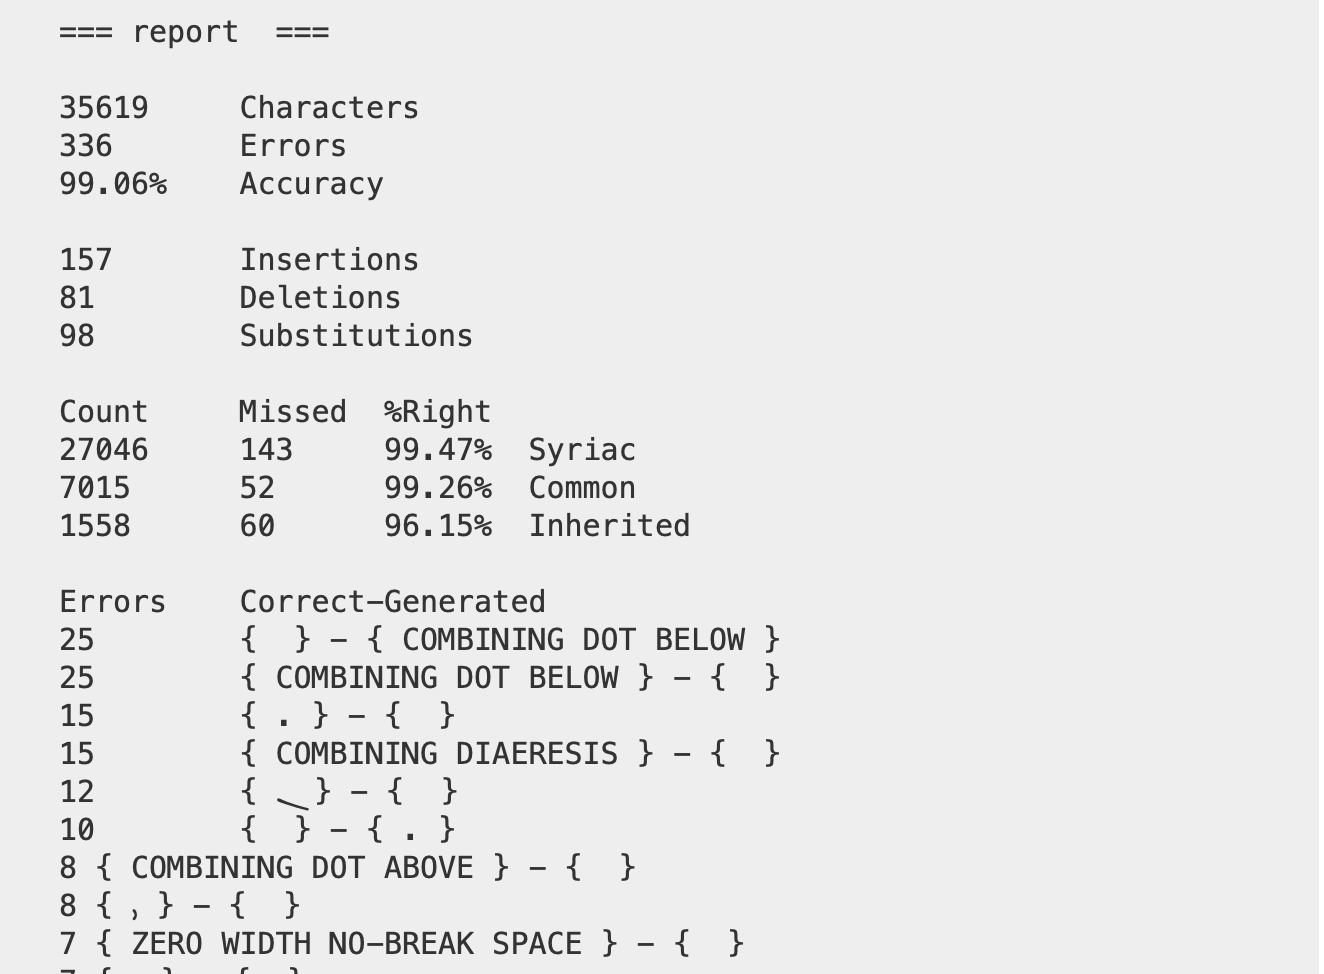
\includegraphics[width=10cm]{images_partie_3/rapport_kraken.png}}}
    \caption{Exemple de rapport fourni par kraken \textcopyright 2015, \cite{noauthor_kraken_nodate}}
    \label{fig:rapport_Kraken}
\end{figure} 

J'ai également voulu vérifier si d'autres outils d'évaluation similaires existaient déjà en parcourant les dépôts de code sur la plate-forme \textit{Github}. J'ai donc relevé trois outils parmi lesquels :  \textit{Werpp}\footnote{\textit{Werpp}, URL : \url{https://github.com/nsmartinez/WERpp}}, \textit{XER}\footnote{\textit{XER}, URL : \url{https://https://github.com/jpuigcerver/xer}} et \textit{WER-in-python}\footnote{WER-in-python, URL : \url{https://github.com/zszyellow/WER-in-python}} à partir de deux fichiers texte brut d'exemples comprenant 10 à 20 mots. 

Le premier représentant un document de vérité terrain, l'autre étant censé montrer la transcription avec des erreurs volontairement insérées (omission de la ponctuation, abus de majuscules, espaces conséquences entre certains mots etc.).\\
\newpage
Une fois les tests effectués, j'ai pu relever les points suivants :
\begin{itemize}
    \item Certains programmes n'utilisaient pas les mêmes versions de Python, comme \textit{Werpp} qui présentait des défauts de compatibilité avec la version 3. Pour le faire fonctionner, il a fallu modifier quelques lignes de codes afin de le rendre exécutable;
    \item Certaines options proposées par ces programmes comme dans \textit{Werpp} ou \textit{XER} ne fonctionnaient pas. Ainsi dans le cas de \textit{XER} le chargement des fichiers au format texte ne fonctionnait pas. Il fallait inscrire les phrases dans le terminal avec une commande du type \citecode{\$ xer -i str -r "Je suis un document valide" -t "je suis Unn DoCument, invalide !"} ce qui n'est évidemment pas du tout envisageable pour des transcriptions de plus de 10 lignes de texte. D'autres options comme la colorisation des résultats pour les lettres manquantes, proposé par \textit{Werpp}, ne fonctionnaient pas en raison de l'obsolescence des \textit{packages} requis;
    \item Certains outils ne permettaient pas de cumuler en sortie plusieurs résultats en même temps comme le WER et le CER. C'est par exemple le cas de \textit{WER-in-python} et de \textit{Werpp};
    \item Enfin les temps de calculs pouvaient s'avérer très longs et la plupart des codes n'étaient pas bien documentés, l'usage des commandes devant être déduites de la lecture du code.\\
\end{itemize}
\medskip

Si la plupart de ces outils ne se sont pas révélés directement utilisables pour notre projet, pour des utilisations fréquentes, ce premier état de l'art m'a permis de me poser des questions quant aux fonctionnalités qui pouvaient être réutilisées et aux métriques qui pourraient s'avérer utiles dans la future application. 

De plus la lecture du code, m'a permis de me familiariser avec la création de CLI par le biais du \textit{package} intégré à Python \textit{argparse}. 

\textit{Argparse} est un \textit{package} Python permettant d'écrire rapidement des programmes sous forme de CLI en récupérant un ensemble de fonctions réutilisables pour permettre entre autre, la gestion des arguments entrés par l'utilisateur dans le terminal, la documentation, etc.\\

Afin de me familiariser avec les logiques de fonctionnement du CLI, j'ai créé un premier programme \citecode{cerwer\_tool}\footnote{Le dépôt du code de l'outil \citecode{cerwer\_tool.py} est disponible sur Github, URL : \url{https://github.com/Lucaterre/cerwer_tool}} en adaptant certaines fonctions des outils décrits plus haut, qui allait préfigurer le développement de l'outil \textit{Kraken-Benchmark} spécifique au projet.\\

L'outil \citecode{cerwer\_tool.py} permettait, en outre, au moyen d'une ligne de commande prenant en argument deux fichiers texte correspondant à une vérité terrain et une prédiction, d'émettre un rapport dans le terminal comportant le nom de l'utilisatrice ou de l'utilisateur, la date, le texte de référence, le texte prédit, de comparer le nombre de mots et de lettres insérées, substituées et supprimées et enfin d'afficher le WER et le CER.

L'utilisatrice ou l'utilisateur avait la possibilité de sauvegarder le rapport dans un fichier texte pour en garder une trace et de produire un graphique présentant le nombre d'insertions, substitutions et de suppressions sur le nombre de mots total (Cf. Figure \ref{fig:cerwer}).\\

Cependant cet outil avait des limites : il supposait de récupérer en amont la transcription HTR, avec \textit{Kraken}, dans un fichier texte pour utiliser \citecode{cerwer\_tool.py}. Comme nous le verrons par la suite, j'ai décidé d'intégrer cette chaîne de traitement HTR directement dans l'outil \textit{Kraken-Benchmark} en réutilisant certaines parties du code de \textit{Kraken} par l'intermédiaire de son API.

\begin{figure}[h]
    \centering
    \centerline{\fbox{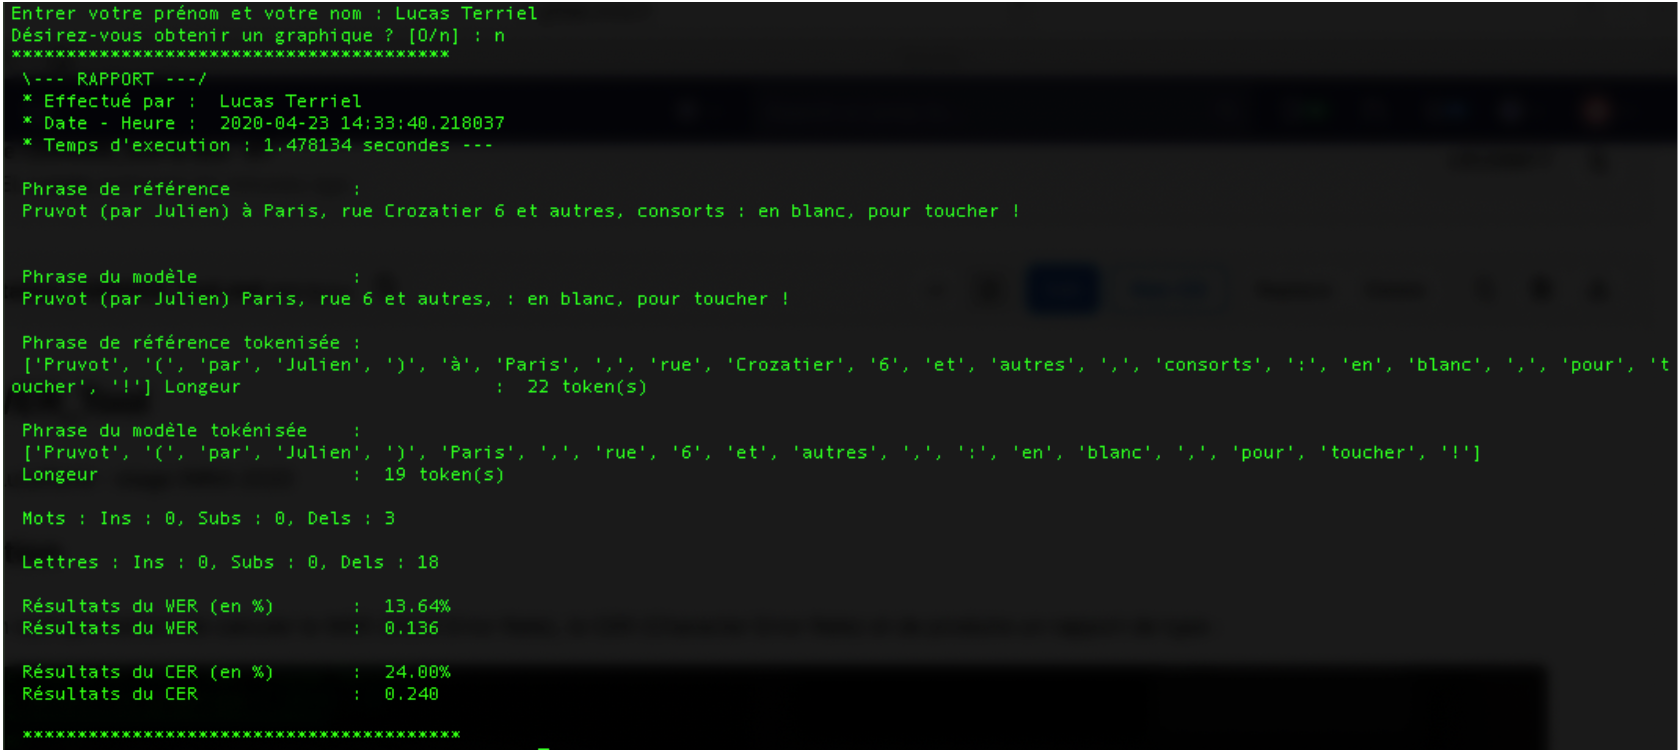
\includegraphics[width=18cm]{images_partie_3/cerwer_tool.png}}}
    \caption{Capture d'écran du rapport produit par le prototype \citecode{cerwer\_tool.py} \textcopyright L. Terriel, 2020, \textit{Pycharm}}
    \label{fig:cerwer}
\end{figure}

\newpage
\section{Des métriques pour comparer la transcription automatique et la vérité terrain}\label{metriques}

Après avoir formulé un état de l'art, je me suis penché sur les méthodes de calcul qui permettent d'évaluer une transcription HTR avec sa vérité terrain. C'est un problème qui peut être ramené à la comparaison de deux chaînes de caractères entres-elles (comparaison \textit{text-to-text}). Dans un deuxième temps, pour permettre d'évaluer les transcriptions dans un contexte de traitement par le TAL, je me suis également intéressé aux métriques permettant d'apprécier la proximité sémantique entre des mots appartenant à deux documents différents.\\

J'ai exposé et synthétisé ce travail de recherche dans un \textit{notebook} Jupyter. Un \textit{notebook} peut être conçu comme un calepin électronique qui permet d'écrire du texte brut et du code au même endroit. Comme nous le verrons par la suite, il est indispensable dans tout travaux concernant le traitement de données en ML et DL, notamment pour expérimenter des calculs, des \textit{scripts} et de préciser certaines étapes\footnote{Le \textit{notebook} de recherche est disponible dans plusieurs formats dans les Annexes \citecode{/C-Application\_Kraken\_Benchmark/Documentation-Reasearch/\\Evaluation de la similarité entre deux séquences dans le contexte de la reconnaissance automatique de caractère} }. Le \textit{notebook} résume brièvement les définitions et les usages des métriques, les visualisations possibles à partir de ces dernières et les différents algorithmes qui permettent de les implémenter dans un programme.\\

\subsection{La comparaison de chaînes de caractères}

Parmi les métriques et les algorithmes associés qui permettent d'évaluer la similarité syntaxique entre deux phrases :\\

\textbf{Le similarité Ratcliff/Obershelp -} L'algorithme de Ratcliff/Obershelp (ou \textit{Gestalt Pattern Matching}) se base sur la recherche de sous-chaînes de caractères communes (\textit{subpattern}) entre deux séquences de caractères.\\

Le principe de l'algorithme de Ratcliff/Obershelp repose sur une découpe des phrases en deux parties en se plaçant par rapport à une ancre qui correspond au premier point de différentiation entre les deux séquences. De part et d'autre, le processus itératif évalue à gauche puis à droite des séquences les plus longues les sous-chaînes communes, jusqu'à ce que la longueur des séquences soit intégralement parcourue.\\
\newpage
La similarité Ratcliff/Obershelp ($ Similarite_{RO} $) calcule deux fois le nombre de caractères effectivement reconnus ($Sub_{caracteres}$) dans les sous-chaînes les plus longues ($\, 2 \cdot Sub_{caracteres} \,$) sur le nombre total de caractères compris dans les deux phrases (signe typographique et espace compris).\\

soit : $$ Similarite_{RO} = \frac{2 \cdot Sub_{caracteres}}{LongChaine_1+LongChaine_2} $$

où : $$ 0 <= Similarite_{RO} <= 1 $$

Par exemple, soit $ S_1 \,= $ \inquote{EN L'AN 1920 PAR LA PROCURATION} et $ S_2 \,=$ \inquote{EN L'AN 1920 PAR LE PROCUREUR}\\

pour $$Similarite_{RO}(S_1 \,, S_2 \,) = \frac{2 \, \cdot \, ([EN\, L'AN\, 1920\, PAR\, L] + [\, PROCUR])}{S_1+S_2} = \frac{50}{60} \simeq  \, 0,83$$\\ 

Dans cet exemple, l'algorithme de Ratcliff/Obershelp trouve dans un premier temps \inquote{EN L'AN 1920 PAR L} à gauche comme la plus longue sous-chaîne commune puis à droite \inquote{ PROCUR} (espace à gauche compris)\footnote{On peut vérifier ce résultat par le biais de deux lignes de code en Python Cf. Annexes, Figure \ref{fig:script_calc_RO}}.\\

Pour inclure ces métriques dans un programme informatique le \textit{package} Python \textit{difflib} permet de récupérer des fonctions qui se basent sur cet algorithme.\\

L'avantage est qu'il permet d'obtenir un score rapidement, afin de comparer deux chaînes de caractères. Cependant elles ne rendent pas compte précisément des modifications de caractères qui ont pu s'opérer lors du passage d'une chaîne à une autre. Nous allons voir en quoi les distances mathématiques peuvent nous y aider.\\
\newpage
\textbf{Les distances de Levensthein, de Hamming et de Damerau-Levenshtein -} La distance de Levensthein\footnote{Établie en 1965 par le mathématicien russe Vladimir Levenshtein (1935-2017)} (équivalent de la distance d'édition), est une distance mathématique, et une généralisation de la distance de Hamming, dans le sens où la première peut travailler sur des chaînes de longueurs différentes, mais pas dans le cas de la seconde.

Cette distance évalue le coût minimal de transformation d'une chaîne de caractères $R$ en une chaîne de caractère $P$ en effectuant les opérations suivantes auxquelles sont associés un coût de 1:

\begin{itemize}
    \item La \textbf{substitution} d'un caractère de $R$ par un caractère de $P$;
    \item L'\textbf{insertion} d'un caractère dans $R$ par $P$;
    \item La \textbf{suppression} d'un caractère dans $R$ par $P$;
\end{itemize}

Pour illustrer le calcul de cette distance nous pouvons prendre les exemples suivants :

\begin{itemize}
    \item soit $R = magasin$ et $P= magasin$, alors $LD(R, P) = 0$, car il n'y a pas de changement.
    \item soit $R = magasin$ et $P= megasinier $, alors $LD(R, P) = 4$, car il eu 3 insertions \inquote{ier} et une substitution \inquote{a} en \inquote{e}. 
\end{itemize} 
\bigskip

La distance de Damerau-Levenshtein\footnote{\cite{chaumartin_traitement_2020}, pp. 132}, quant à elle, est une variation de la distance de Levensthein qui inclut les transpositions (échange de deux lettres) dans les opérations (pour prendre en compte les fautes d'orthographe ou les échanges de caractères).

Par exemple dans le cas des mots \inquote{acceuil}, \inquote{auteuil} et \inquote{accueil}, la distance de Levensthein calcule une distance de 2 entre chaque mots. Cependant \inquote{acceuil} et \inquote{accueil} sont plus proches (transposition de \inquote{eu} en \inquote{ue}) que \inquote{auteuil} et \inquote{acceuil}, la distance de Damerau-Levenshtein prend en compte cette différence. Ainsi la modification \inquote{acceuil} et \inquote{accueil} sera pondéré à 1 tandis que la modification \inquote{auteuil} et \inquote{acceuil} sera pondéré à 2. Une transposition de deux caractères coûte moins qu'une substitution. 

Cette distance est plutôt utilisée dans le cadre de correcteur orthographique, de plus la complexité algorithmique de la distance de Damerau-Levenshtein est plus élevée que la distance de Levensthein, ce qui est une caractéristique à prendre compte durant l'implémentation. La distance de Damerau-Levenshtein sera plus longue à calculer que la distance de Levensthein (environ 20 secondes pour la première et 0,01 secondes pour la seconde (implémentation la plus rapide) pour des chaînes d'environ 350 caractères).\\

Il existe plusieurs algorithmes pour implémenter cette distance\footnote{\cite{wikibooks_algorithm_2020}}; la tâche d'implementation peut être facilité par des \textit{packages} en Python, comme la fonction \citecode{\_fast\_levenshtein()} de l'API de l'\textit{Kraken}\footnote{\cite{noauthor_kraken_nodate}} ou encore  \textit{python-levenshtein}\footnote{\cite{noauthor_python-levenshtein_nodate}} qui est une implantation plus rapide de la distance (extension écrite en langage C).\\

Nous allons voir que cette distance est importante si on veut pouvoir calculer le taux d'erreur par caractères (CER) et le taux d'erreur par mots (WER).\\ 

\textbf{Le taux d'erreur de caractères et le taux d'erreur de mots -} Le taux d'erreur de caractères (\textit{Character error rate} ou CER) et le taux d'erreur de mots (\textit{Word error rate} ou WER) sont des taux d'erreurs très utilisés pour constater l'efficacité d'un modèle de reconnaissance. Le CER et le WER se calcule de la manière suivante :

Si : 

\begin{itemize}
    \item $N$ est le nombre total de caractères ou de mots contenus dans la phrase de référence;
    \item $S$ (\textit{Substitution}) est le nombre de substitutions (mots ou caractères incorrectement reconnus);
    \item $D$ (\textit{Deletion}) est le nombre de suppressions (mots ou caractères omis);
    \item $I$ (\textit{Insertion}) est le nombre d'insertions (mots ajoutés).
\end{itemize}

Le CER se calcule tel que : $$ Character\, Error\, Rate = \frac{S\, + \,D\, + \,I\,}{N_{total\, de\, caracteres}} $$

Le WER se calcule tel que : $$ Word\, Error\, Rate = \frac{S\, + \,D\, + \,I\,}{N_{total\, de\, mots}} $$

Dès lors si on connaît la distance de Levensthein $D$ pour une phrase de référence notée $R$ et une phrase de prédiction $H$, le CER peut être ramené à l'expression suivante : $$CER = \frac{D(R,H)}{N_{total\, de\, caractères}}$$  et le WER :$$WER = \frac{D(R,H)}{N_{total\, de\, mots}}$$

Les résultats obtenus sont interprétés de la sorte : plus le taux approche 0 plus la reconnaissance est efficace, à l'inverse, plus le taux se rapproche de 1, plus le texte a eu du mal à être reconnu. Il peux même dépasser 1, si la reconnaissance est très mauvaise, surtout s'il y a eu beaucoup d'insertions. Nous avons été confronté à ce cas, comme nous le verrons en chapitre \ref{tests_KB_lectaurep}. Notons enfin qu'il est possible de ramener ces taux d'erreurs à des pourcentages pour une meilleure visibilité.\\

A partir du WER on peut également calculer le taux de reconnaissance de mots (ou \textit{Word Accuracy} (WAcc)), calculé pour obtenir un pourcentage de la manière suivante (à noter que le résultat peut-être négatif si le WER dépasse 1): $$W_{ACC}\, = (1 - WER) \cdot 100  $$

Le CER est plus significatif que le WER et que le taux de reconnaissance par mots dans le sens où ces derniers sont corrélés aux erreurs de prédiction des caractères effectués par le modèle. \textit{De facto} le WER augmente et le taux de reconnaissance par mots baisse quand le CER augmente. Cependant, dans un projet HTR ces métriques peuvent se compléter; ainsi il est intéressant de savoir si un modèle qui fait beaucoup de fautes épargne les mots et à l'inverse si un modèle fait peu de fautes, ci ces dernières se retrouvent sur tous les mots.

\subsection{Estimer la similarité entre deux documents}

L'intuition est de prendre la vérité terrain comme premier document et sa prédiction par le modèle HTR comme un deuxième document. L'indice de Jaccard ainsi que la similarité cosinus sont des métriques qui évaluent la proximité entre des textes :\\

\textbf{L'indice de Jaccard -} Son but est d'estimer le pourcentage de mots communs aux deux documents. L'indice évalue, sur l'union de deux ensembles (deux phrases par exemple), la taille de l'intersection qui regroupe les mots commun à la transcription de référence et à la transcription HTR, qu'il divise par la taille de l'union de deux ensembles.

L'indice est formulé ainsi : $$ J(doc_1,doc_2) = \frac{|doc_1 \cap doc_2|}{|doc_1 \cup doc_2|} $$

Plus le résultat approche de 1, plus les documents sont similaires, car le nombre des mots partagés par la référence et par sa transcription HTR dans l'intersection est important. À l'inverse, si le résultat est plus proche de 0, alors on peut en conclure que les deux textes sont davantage éloignés l'un de l'autre.\\

\textbf{La similarité cosinus -} Si l'on reprend la Figure \ref{fig:word_embedding} à la section \ref{TAL_repertoire}, il s'agit de calculer l'angle cosinus noté $cos(\theta)$ entre des mots, alors représentés sous la forme de vecteurs, afin de mesurer leur degré de proximité. La formule de la similarité cosinus est la suivante : $$ similarite\, cosinus \, = cos\, (\theta\,) = \frac{\overrightarrow{V1}\, \cdot \,\overrightarrow{V2}}{||\overrightarrow{V1}||\, \cdot \,||\overrightarrow{V2}||} $$

où : 

$$ ||\overrightarrow{V1}||\, et\, ||\overrightarrow{V2}||\, >\, 0 $$

Les résultats obtenus sont interprétés de la manière suivante, en fonction de la valeur de $cos(\theta)$ :

\begin{itemize}
    \item Plus elle tend vers 0, plus les vecteurs sont dits indépendants ou opposés (orthogonaux) : les documents sont donc éloignés;
    \item Plus elle tend vers 1, plus les vecteurs sont dits (colinéaires de coefficient positif) donc les documents sont proches;
\end{itemize}

Pour illustrer cette métrique prenons un exemple concret issu d'un répertoire de notaire. En nous appuyant sur une vérité terrain ($R$ pour référence) et une prédiction ($P$) réalisées par un modèle de transcription qui a émis quelques erreurs.\\

$R$ = \inquote{An 1920, mois d'Avril pour gerer 2 maisons à Paris Procuration, par Rosalie Adélaïde Eugénie Isoarel, dt à Paris, rue de la Collégiale}\\

$P$ = \inquote{sAn 19s2iOt, mois de Avril per gerer 2ts maisons à Paris Procuration, par Reselie Adelaide Eugenie lisrel, dt a Peres, rue de la Collégiale}\\

Leurs termes sont : \inquote{an, mois, avril, gerer, maisons, paris, procuration, roasalie, adélaïde, reselie, adelaide, eugénie, eugenie, isoarel, isrel, rue, collegiale}\\

On pourra alors représenter $R$ et $P$ sous forme de vecteurs à 17 dimensions (correspondant au nombre de termes relevés) dont les valeurs numériques représentent les occurrences d'apparition du mot dans la phrase :

$$R\,=\,[1,1,1,1,1,2,1,1,1,0,0,1,0,1,0,1,1]$$
$$P\,=\,[0,1,1,1,1,1,1,0,0,1,1,0,1,0,1,1,1]$$

Si la norme du vecteur $R$ se calcule tel que : $$||\overrightarrow{R}|| = \sqrt{R_1 \cdot R_1 + R_2 \cdot R_2 + \ldots + R_n \cdot R_n}$$

On aura donc $||\overrightarrow{R}|| = 4.0 $ et $||\overrightarrow{P}|| = 3.46 $

Le produit scalaire de $R \cdot P$ se calcule tel que : $$R \cdot P = R_1 \cdot P_1 + R_2 \cdot P_2 + \ldots + R_n \cdot P_n$$

On aura donc $R \cdot P = 9$

Dès lors, si la formule de la similarité cosinus s'exprime tel que : $$SimCos(R,P) = \frac{R \cdot P}{||\overrightarrow{R}|| \cdot ||\overrightarrow{P}||}$$

On obtient alors le résultat suivant : $SimCos(R,P) = 9 / (4.0 \cdot 3.46) = 0.65$ \\ On peut dire que les documents sont éloignés dès lors le modèle à commis des erreurs (un écart d'environ 35\%).

\subsection{Remarques complémentaires sur les métriques d'évaluation utilisées}

Au vue des différentes métriques présentées, j'ai décidé de travailler sur deux types de métriques dans l'application \textit{Kraken-Benchmark} afin d'évaluer la correspondance entre deux phrases.

Une première catégorie de métriques, de type \inquote{similarité sémantique}, empruntées à la fouille de textes, va chercher à savoir si les mots généraux ou les entités nommées (lieux, personnes ou types d'actes) sont équivalents dans les deux textes et sont donc bien reconnus par le modèle. C'est le cas de la similarité cosinus et de l'indice de Jaccard. Cependant, il s'agit d'une utilisation non conventionnelle dans le cadre de l'évaluation HTR de ces métriques qui évaluent la proximité sémantique d'un grand ensemble de documents. De plus, elles ne seront pas assez précises pour savoir si les deux phrases sont strictement équivalentes et syntaxiquement correctes car pour se calculer ces métriques nécessitent souvent qu'on enlève les mots fréquents (\textit{stops words}) qui peuvent également contenir des fautes de transcription (qui sont intéressants à relever si l'on veut obtenir une bonne qualité de transcription) pour réaliser une représentation de type \inquote{sac de mots} (\textit{bag of words}) et obtenir un modèle vectoriel des textes (\textit{word embedding}).

Les métriques, dites de \inquote{similarité syntaxique}, travaillent, quant à elles, sur la position exacte des mots et des caractères dans la phrase. Elles nous apporteront des précisions sur les types de modifications qui ont été le plus souvent opérées par le modèle. Il s'agira des métriques \inquote{classiques} de l'HTR comme la distance de Levensthein, le CER et le WER.

Il faut noter que pour permettre l'implémentation de ces métriques dans un programme informatique des étapes de normalisation des données textuelles sont requises : on parle de \textit{data pre-processing}. On a donc eu recours durant le développement de l'application à des fonctions de découpage des phrases en caractères ou en mots (\textit{tokenisation}), de suppression des mots les plus fréquents (\textit{stops words}), ainsi que des moyens de convertir les mots sous formes de valeurs numériques, comme la transformation en vecteurs (\textit{word embedding}).\\

Pour terminer cette section, il est possible de retrouver dans le \textit{notebook} intitulé \inquote{Évaluation de la similarité entre deux séquences dans le contexte de la reconnaissance automatique de caractères} davantage de précisions sur les métriques, les étapes de normalisation du texte, leurs différentes implémentations en Python, des tests de durée d'exécution et les visualisations réalisées (graphiques, matrices de confusion etc.) (Cf. Annexes \ref{annexe_KB}).\\
\clearpage
\thispagestyle{empty}
\chapter{Le développement d'une application : Kraken-Benchmark}

\section{Modélisation}

\subsection{Les objectifs fixés au début du développement}\label{objectifs}
En concertation avec ma tutrice de stage, Alix Chagué, j'ai fixé des cas d'usages (\textit{use case}) et formalisé les objectifs idéaux à atteindre dans la conception de l'application. Ceci dans l'optique de  décrire les exigences fonctionnelles de la future application. Nous avons donc relevé que :

\begin{itemize}
    \item L'application doit pouvoir comparer et évaluer la qualité d'un modèle de transcription et/ou de segmentation à l'échelle d'une ou de plusieurs images;
    \item Les résultats de l'évaluation doivent être accessibles et visualisables dans une interface conviviale pour l'utilisateur (\textit{user-friendly});
    \item Le rapport produit doit pouvoir être exporté dans plusieurs formats;
    \item L'utilisateur doit avoir la possibilité de charger les images et le modèle facilement;
    \item Le programme doit être écrit en Python 3 pour assurer sa  maintenabilité dans le temps;
    \item Le code, et l'application, doivent disposer d'une documentation interne et externe;
    \item Le programme doit pouvoir être généralisé à d'autres projets et/ou viser une interropérabilité avec la plate-forme \textit{eScriptorium} à terme;
\end{itemize}

Nous verrons dans la section \ref{perspectives_amélios} les objectifs qui ont été atteints, ceux qui restent en cours de développement et ceux qui ont émergés au cours des tests et rédaction du code. 

\subsection{Un écosystème Python orienté pour la science des données et la conception d'application \textit{web}}

Pour réaliser l'application \textit{Kraken-Benchmark} en Python \footnote{l'ensemble des fichiers de l'application cités à partir de maintenant sont disponibles dans les Annexes \ref{annexe_KB}}, il m'a fallut disposer de solutions pour concevoir l'interface, mais aussi pour effectuer des tâches plus précises comme les calculs et les représentations graphiques de données (\textit{data visualisation}). Quand il s'agit d'évaluer des données, Python fait graviter autour de lui un ensemble d'outils orientés pour la science des données (\textit{data science}, Cf. Figure \ref{fig:eco_datascience}) comprenant la manipulation et la fouille de données, des statistiques, des visualisations, l'application de modèles mathématiques, et l'apprentissage automatique. 

\begin{figure}[h!]
    \centering
    \centerline{\fbox{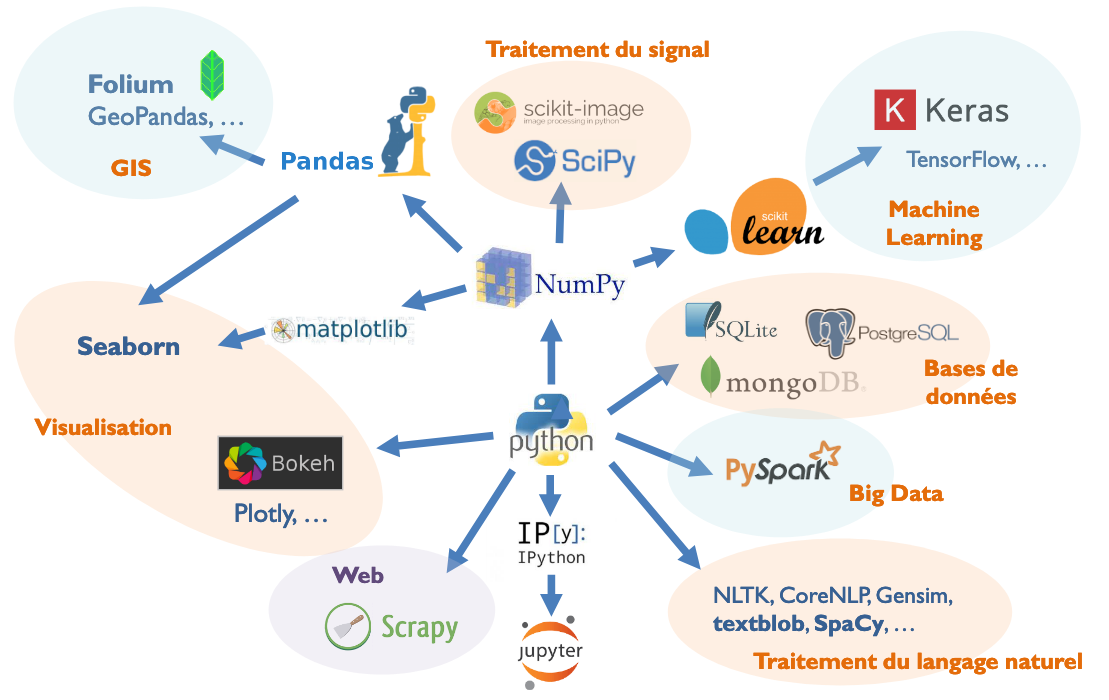
\includegraphics[width=15cm]{images_partie_3/ecosysteme_datascience.png}}}
    \caption{L'écosystème Python pour la science des données (\textit{datascience})   \textcopyright F.Pennerath, Mineure \inquote{Data Science}, Centrale Supélec}
    \label{fig:eco_datascience}
\end{figure}

Pour fonctionner et effectuer des traitements, l'application \textit{Kraken-Benchmark} requiert, outre le langage Python 3, l'installation des \textit{packages} suivants (certains ont déjà étaient aperçus dans les sections précédentes et d'autres étant déjà inclus dans le langage Python) : 
\newpage
\begin{itemize}
    \item Pour réaliser les calculs et l'implémentation des \textbf{métriques d'évaluation} : \textit{Sklearn}\footnote{\cite{noauthor_scikit-learn_nodate}}, \textit{Numpy}\footnote{\cite{noauthor_numpy_nodate}}, \textit{Python-Levenshtein}\footnote{\cite{noauthor_python-levenshtein_nodate}}, \textit{Kraken API}\footnote{\cite{noauthor_kraken_nodate}}, et des \textit{packages} inclus dans Python comme \textit{difflib}, \textit{math}, \textit{collections};
    \item Pour réaliser les \textbf{visualisations de données} : \textit{Matplotlib}\footnote{\cite{noauthor_matplotlib_nodate}}, \textit{Seaborn}\footnote{\cite{noauthor_seaborn_nodate}}, Pandas\footnote{\cite{noauthor_pandas_nodate}};
    \item Pour le \textbf{pré-traitement des données textuelles} (découpage des phrases en mots et suppressions des mots les plus fréquents) : \textit{NLTK}\footnote{\cite{noauthor_nltk_nodate}}
\end{itemize}

À coté de ses \textit{packages} orientés science des données, j'ai eu besoin de recourir à des \textit{packages} plus spécifiques : 

\begin{itemize}
    \item Traitement des images en entrée : \textit{Pillow}\footnote{\cite{noauthor_pillow_nodate}};
    \item Réalisation de la chaine de traitement HTR : \textit{Kraken API};
    \item Gestion de la partie CLI : \textit{argparse};
    \item Gestion de la partie GUI (\textit{Graphical User Interface}) de l'application dans le navigateur \textit{web} : \textit{Flask}\footnote{\cite{noauthor_flask_nodate}}
\end{itemize}

Initialement au début du projet il était prévu de n'utiliser que le moteur de \textit{templates}\footnote{Un moteur de \textit{templates} permet de séparer la partie traitement pur des données en Python de la partie visuelle de l'application. Le \textit{template} d'un projet \textit{web} contiendra tous les fichiers HTML (pour la structure), le CSS et les images (style et aspect visuel du site), et le Javascript (pour les animations).} \textit{Jinja}\footnote{\cite{noauthor_jinja_nodate}}. Cependant, j'ai rapidement constaté les limites, notamment quand je devais permettre à l'utilisatrice ou à l'utilisateur de pouvoir accéder à plusieurs pages dans le navigateur (plusieurs vues), un gestionnaire de \textit{templates} seul n'était pas suffisant. 

L'avantage de \textit{Flask} repose sur le fait qu'il s'agit d'une boîte à outils (mini \textit{framework} \textit{web}) pour construire des applications \textit{web}. Ainsi en plus d'intégrer le moteur de \textit{templates} \textit{Jinja}, il intègre également un gestionnaire de routes (les différentes routes URL pour définir les vues), et dispose d'un gestionnaire de requêtes HTTP ainsi que d'un serveur de développement\footnote{On distingue le serveur de développement, pour tester les applications \textit{web}, du serveur de production, qui permet de déployer et d'installer l'application \textit{web} finalisée qui est donc accessible aux utilisateurs.} pour tester l'application\footnote{\textbf{HTTP} (HyperText Transfer Protocol), est un protocole de communication entre client et serveur pour le \textit{web}.} et pour communiquer avec le code Python (ou WSGI\footnote{WSGI ou \textit{Web Server Gateway Interface}, est interface entre des serveurs et des applications \textit{web} pour Python. c'est une spécification qui permet à l'application Python de recevoir une requête HTTP transformée en un objet Python et de retourner une réponse HTTP sous la forme d’un autre objet Python également.}) \textit{Werkzeug}\footnote{\cite{noauthor_werkzeug_nodate}}.\\

La structuration des éléments de texte (titres, description, paragraphes) de l'interface graphique a été réalisé à partir des \textit{templates} \textit{Jinja}, qui permettent de faire des appels d'objets Python directement dans le fichier HTML pour y insérer d'autres éléments comme les métriques. L'apparence générale du site (fenêtre principal, boutons, formulaires, bannière etc.) repose sur le \textit{framework} \textit{Bootstrap}\footnote{\cite{otto_bootstrap_nodate}} qui est une collection d'outils de stylisation pour les sites \textit{web} qui contient une feuille de style CSS déjà écrite. De plus, afin de rendre le site plus dynamique (symboles de chargement (\textit{loader}), apparition des éléments au défilement etc.), j'ai ajouté des scripts en JQuery à la fin des pages HTML\footnote{JQuery est une bibliothèque JavaScript pour faciliter l'écriture de scripts côté utilisatrices ou utilisateurs.}.\\

La plupart des \textit{packages} Python listés ci-dessus sont disponibles avec la distribution Python \textit{Anaconda}. Il s'agit d'une distribution de Python comprenant le langage Python 3 mais également un ensemble de \textit{packages} dédiés à la science des données. Ainsi plutôt que de devoir installer les \textit{packages} un à un via le gestionnaire de base \textit{pip}\footnote{\textbf{pip} est le gestionnaire de \textit{packages} Python par défaut. Il permet d'installer des \textit{packages} supplémentaires dans la distribution Python classique par l'intermédiaire d'une commande de type \citecode{pip install nom-du-paquet}.}, l'utilisateur pourra créer un environnement virtuel \textit{conda} par le biais du fichier \citecode{environment.yml} qui regroupe les \textit{packages} cités plus haut.\\ 

L'installation et les commandes pour utiliser l'application sont résumés dans un fichier de type \inquote{lisez-moi} (\citecode{README.md}).
\newpage
\subsection{Les étapes de fonctionnement : retour sur quelques aspects de programmation}

Après avoir rassemblé les outils pour réaliser le programme, j'ai modélisé les différentes étapes qu'il devait réaliser. De la même manière que pour développer l'outil \textit{Generator Lectaurep-TEI} abordé dans la section \ref{generator-lecto-dev}, j'ai créé un modèle résumant l'algorithme de l'application (Cf. Annexes, Figure \ref{fig:algo-kb}).\\

Le programme se résume aux étapes suivantes :
\begin{enumerate}
    \item Avant de lancer, l'utilisatrice ou l'utilisateur place dans différents dossiers les fichiers à traiter. À la racine du \textit{script} principal \citecode{kraken\_benchmark.py} l'utilisatrice ou l'utilisateur peut créer le dossier \citecode{dataset\_GT} qui reçoit les fichiers en texte brut de la vérité terrain, le dossier \citecode{images} qui reçoit les images (format .jpeg) à reconnaître, et dans le dossier \citecode{model} un modèle (.mlmodel) pré-entraîné avec \textit{Kraken}. L'utilisatrice ou l'utilisateur doit conserver le même ordre de fichiers dans les dossiers \citecode{dataset\_GT} et \citecode{images} en utilisant un label dans le nommage de fichiers. Ainsi les images pourront être notées \citecode{image\_1, image\_2 \ldots} et les transcriptions correspondantes \citecode{transcription\_1, transcription\_2 \ldots} Sans cet étiquetage le programme risque d'associer une image avec la mauvaise transcription et la mauvaise vérité terrain.\\
    \item Une fois l'étape précédente réalisée, on peut lancer le programme via la commande \citecode{\$ python kraken\_benchmark.py}. L'utilisatrice ou l'utilisateur peut également spécifier des options derrière sa commande comme \textbf{-{}-label} s'il ou si elle souhaite renseigner des métadonnées sur ces images, \textbf{-{}-verbosity} s'il ou si elle souhaite avoir un rapport complet durant chacune des étapes du programme, et une option \textbf{-{}-clean\_text} qui permet, en outre, d'enlever la ponctuation et les caractères non alphabétiques, ce qui peut être utile pour certains types de projets.\\
    \item Le \textit{script} principal \citecode{kraken\_benchmark.py} lance une première étape de transcription HTR (qui s'appuie sur les fonctions des modules de l'API \textit{Kraken}). Après avoir associés les images avec leur transcription vérité terrain, le programme effectue le processus suivant : il charge le modèle de transcription et les images, les images sont binarisées, il procède ensuite à la segmentation des images pour repérer les coordonnées des lignes de textes et effectue les prédictions qui sont normalisées dans un encodage UTF-8;
    \item Le \textit{script} principal \citecode{kraken\_benchmark.py} rassemble alors, par triplet : l'image, la vérité terrain et la prédiction;
    \item Chacun des triplets est transformé en objet \citecode{SynSemTS} appartenant au module \citecode{SynSemTS.py} sur lesquels on peut récupérer les différentes métriques et visualisations associées;
    \item Le groupe d'objets est alors récupéré par le module \citecode{kb\_report} qui prend le relais et se charge d'ouvrir le navigateur \textit{web} automatiquement sur un serveur de développement par défaut;
    \item L'utilisatrice ou l'utilisateur peut alors circuler dans l'application et afficher les différentes pages \textit{web}. Le \textit{script} \citecode{routing.py} du dossier \citecode{kb\_report} est chargé d'envoyer et de recevoir les requêtes URL pour afficher la page HTML correspondante durant la navigation de l'utilisatrice ou de l'utilisateur, jusqu'à la fin de la session.
\end{enumerate}

Dans les sections qui suivent nous avons souhaité relater quelques questions de programmation rencontrées au cours du développement de l'application, plutôt que de simplement montrer le code Python brut. 
Le code source de l'application est consultable dans l'Annexe \ref{annexe_KB}, et une documentation interne au code explicite le rôle de chaque fonctions codés sous la forme de \textit{docstrings}\footnote{Les \textit{docstrings} sont des chaînes de texte situées à certains endroits du code pour commenter ou documenter. Elles visent à rendre le code source plus explicite pour les personnes qui souhaiteraient le réutiliser ou le maintenir. Elles peuvent suivre des conventions comme la PEP 257, le modèle \textit{Sphinx}, ou le style \textit{Google Python}.}. 

\subsubsection{Un jeu de données pour réaliser des tests fonctionnels}

Durant le développement de l'application, je devais disposer de transcriptions de vérité terrain et d'un modèle de transcription pour tester l'application au fur et à mesure des ajouts de fonctionnalités. J'ai constitué un jeu de données en me basant sur des extraits de l'ouvrage \textit{Voyage au centre de la Terre} de Jules Verne (dossier \citecode{jules\_verne\_set\_test}). Toutefois, il ne s'agissait pas de réaliser un OCR de qualité, mais simplement de récupérer des données de tests à passer dans l'application.

Dans un premier temps, j'ai trouvé sur Gallica\footnote{Bibliothèque numérique de la Bibliothèque nationale de France} une série de 8 images hétérogènes. Parmi celles-ci, certaines contenaient du texte imprimé sur toute la page et d'autres des illustrations, de tailles variables, dans l'optique de tester ces différences. 

La deuxième étape a été de constituer des vérités terrains en me basant sur l'environnement de transcription de \textit{Kraken}\footnote{Précisons qu'il s'agit d'un environnement \inquote{dépassé} qui n'est plus compatible avec la dernière version de \textit{Kraken} mais qui reste suffisant pour générer du texte.} (Cf. Figure \ref{fig:transcrire_kraken}). 

Après avoir lancé la ligne de commande correspondante, le canevas de transcription apparaît sur une page HTML qui comprend, à gauche l'image et à droite les lignes à transcrire. Cela peut s'apparenter à une version minimaliste de la plate-forme \textit{eScriptorium}.   

\begin{figure}[H]
    \centering
    \centerline{\fbox{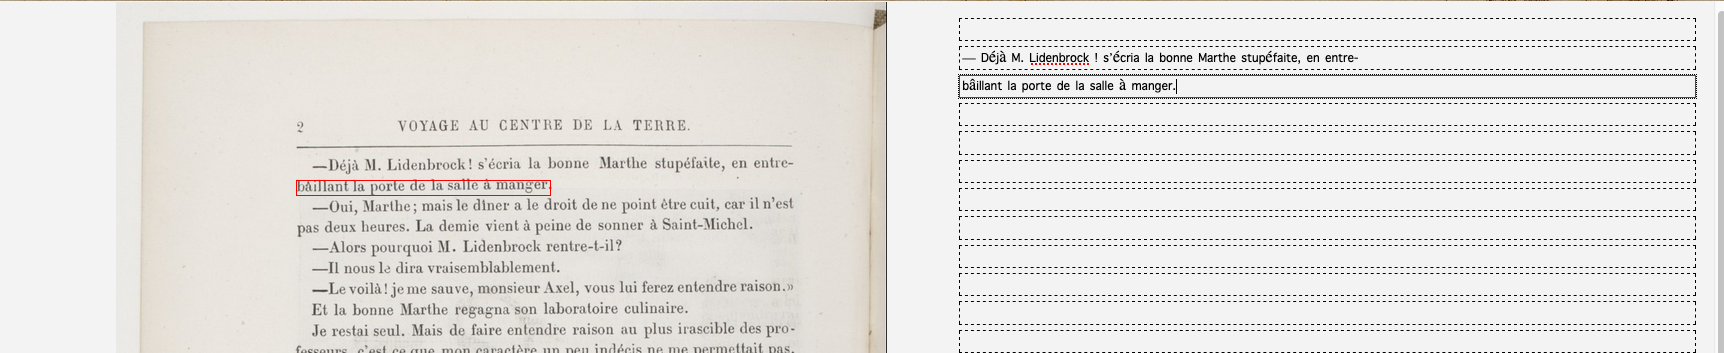
\includegraphics[width=19cm]{images_partie_3/transcrire_kraken.png}}}
    \caption{Environnement de transcription de Kraken utilisés pour créer des vérités terrains de tests \textcopyright L. Terriel, 2020, \textit{Kraken}}
    \label{fig:transcrire_kraken}
\end{figure}

Une fois les transcriptions effectuées, une ligne de commande permet de récupérer les données d'entraînement avec \textit{Kraken} sous la forme de fichier texte (le nommage du fichier étant de la forme \citecode{image\_transcrite\_1.gt.txt}) dans le dossier où l'on se situe. La dernière étape consistait par le biais d'une autre ligne de commande à entraîner un modèle de transcription à partir des vérités terrains constituées. Le modèle à pu être entraîné rapidement et les derniers résultats obtenus étaient plutôt satisfaisants (en cause les écritures imprimées lisibles). 

\subsubsection{Deux niveaux d'interface pour un prototypage rapide}

La volonté de me concentrer rapidement sur la partie permettant d'exposer les métriques dans le navigateur et de disposer d'un outil, avant la fin du stage, pour effectuer des tests avec les données spécifiques de Lectaurep, m'ont obligé à faire un certain nombre de choix techniques. 

Dans la mesure où il s'agit d'un prototype expérimental et interne à ALMAnaCH, il ne m'a pas paru nécessaire de doter l'application d'une interface graphique la partie chargement des données, traitement HTR/OCR, pré-traitements des données textuelles, et calculs. \\

J'ai séparé dès le départ :

\begin{itemize}
    \item Une partie CLI, qui repose sur le \textit{script} principal \citecode{kraken\_benchmark.py} contenant la fonction chargée de réaliser la partie HTR. Ce \textit{script} est relié à un module pour des traitements plus spécifiques \citecode{kraken\_utils.py} : récupération du chemin des fichiers, impressions des messages de succès ou d'erreurs, construction de structures de données Python spécifiques, ou encore récupération des images dans le dossier \citecode{static} pour les afficher dans le navigateur. Le dossier \citecode{STS\_Tools}, qui s'apparente à une \inquote{mini libraire} contient  deux modules \citecode{SynSemTS.py} et \citecode{STSig.py} qui sont utilisés pour construire des objets sur lesquels on peut retrouver les métriques et les visualisations graphiques, dans le but de les afficher dans le navigateur (nous reviendrons sur la spécificité de ces deux modules);\\
     \item Une partie GUI axée sur l'affichage dans le navigateur des métriques et des visualisations par l'ouverture du serveur de développement, le système de gestion des routes URL et des pages HTML par le module \citecode{routing.py} dans le dossier \citecode{kb\_report} qui est appelé à l'issue du \textit{script} principal \citecode{kraken\_benchmark.py}. 
\end{itemize}
\bigskip
Enfin, j'ai tenté de rendre l'affichage dans le terminal, pour la partie CLI, suffisamment convivial et explicite grâce à des \textit{packages} Python. L'objectif étant que l'utilisatrice ou l'utilisateur puisse avoir des informations sur les étapes en cours. Chaque étape dispose d'une barre de progression qui indique le temps de traitement (\textit{tqdm}\footnote{\cite{noauthor_tqdm_nodate}}), une colorisation indique bien à l'utilisatrice ou l'utilisateur les messages d'erreurs et les messages de succès (\textit{termcolor}\footnote{\cite{noauthor_termcolor_nodate}}) et un affichage stylisé et une indication sonore alerte l'utilisatrice ou l'utilisateur que le programme est en attente d'informations (\textit{prompt\_toolkit}\footnote{\cite{noauthor_prompt-toolkit_nodate}}). 

\subsubsection{La programmation orientée objet : une solution pour généraliser et mieux documenter le code}
Au fur et à mesure du développement de l'application la nécessité de rassembler les fonctions de calculs des principales métriques\footnote{Décrites pour la plupart en section \ref{metriques}} en dehors du \textit{script} principal \citecode{kraken\_benchmark.py} s'est fait ressentir. En effet celui-ci se surchargeait de fonctions et la clarté du code devenait plus difficile à maintenir.\\ 

Le recours à la programmation orientée objet (POO), rendue possible par Python, a été un bon moyen de contourner le problème et cela pour plusieurs raisons. Cependant, pourquoi ne pas avoir pris le parti de mettre les fonctions métriques dans un module comme \citecode{kraken\_utils.py} qui regroupe des fonctions annexes au \textit{script} principal ?\\ 

Les paragraphes suivants ont pour but de présenter brièvement la programmation objet, qui n'a pas la prétention de résumer un sujet aussi vaste, mais uniquement de cerner les enjeux, pour en venir à son utilisation concrète et à ses avantages pour l'application.
\newpage
La programmation objet est un paradigme de programmation qui consiste à structurer une application sur la base d'un assemblage d'entités indépendantes reliées entre-elles. C'est entités sont appelées \inquote{objets}. On peut voir un objet comme un concept du monde réel possédant des caractéristiques (en Python, on parle de propriétés), des comportements (méthodes), et peuvent avoir des interactions avec d'autres objets (Cf. Figure \ref{fig:concept_POO}). 
\begin{figure}[H]
    \centering
    \centerline{\fbox{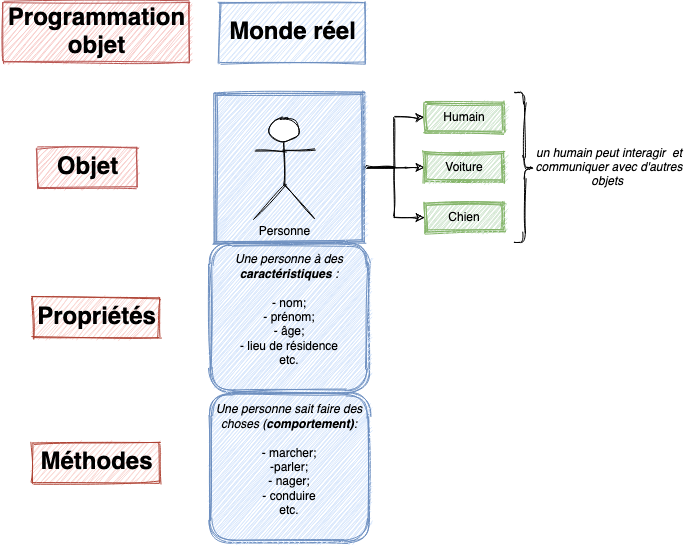
\includegraphics[width=16cm]{images_partie_3/concept_POO.png}}}
    \caption{Le concept de personne peut être représenté sous la forme d'un objet \textcopyright L. Terriel, 2020, Diagrams.net}
    \label{fig:concept_POO}
\end{figure}
\newpage
Un objet peut relever d'une même catégorie. Ainsi une voiture est une sorte d'objet avec des caractéristiques et des méthodes propres pouvant appartenir à la catégorie moyen de transport. Celle-ci peut être modélisée au moyen d'une classe en langage orienté objet. La classe est apparentée à une usine qui va créer des objets héritant des propriétés de cette classes. L'exemple de code ci-dessous montre le moyen de créer un objet \inquote{Personne} en Python :

\lstset{language=Python}
\begin{lstlisting}
"""On définit une classe Personne"""
class Personne:
    def __init__(self, nom, prenom, age, lieu):
        """Le constructeur permet de placer les propriétés de l'objet"""
        self.nom = nom
        self.prenom = prenom
        self.age = age
        self.lieu_de_naissance = lieu
        """propriétés spécifiques pour les actions de l'objet"""
        self.nombre_de_pas = 0
    """On donne des comportements aux objets (méthodes)"""
    def marcher_en_avant(self):
        self.nombre_de_pas += 1
        return print(f'{self.prenom} {self.nom} a fait {self.nombre_de_pas} pas !')
    def parler(self, mot):
        return print(f'mon mot est : \"{mot}\"')

"""On créé un objet Personne (instanciation de l'objet dans la classe Personne)"""
Personne_1 = Personne("Mabillon", "Jean", 388, "Saint-Pierremont")

"""On peut vérifier l'objet créé"""
print(Personne_1)
>>> <__main__.Personne object at 0x1013862d0>

"""On peut récupérer des propriétés de l'objet"""
print(Personne_1.prenom)
>>> Jean

"""On peut faire agir l'objet"""
Personne_1.marcher_en_avant()
>>> Jean Mabillon a fait 1 pas !
Personne_1.parler('De re diplomatica')
>>> mon mot est : "De re diplomatica"
\end{lstlisting}

C'est cette technique de programmation que j'ai mis en pratique afin de créer les deux modules \citecode{SynSemTS.py} et \citecode{STSig.py}. Nous aurons l'occasion de revenir sur ce dernier module d'expérimentation créé pour tester de nouvelles métriques et qui est encore en phase de développement, dans la section \ref{inter_fonc}.\\

Le diagramme présenté en figure \ref{fig:diag_synsem}, ci-dessous, montre les différentes classes du module 
\citecode{SynSemTS.py}.

\begin{figure}[H]
    \centering
    \centerline{\fbox{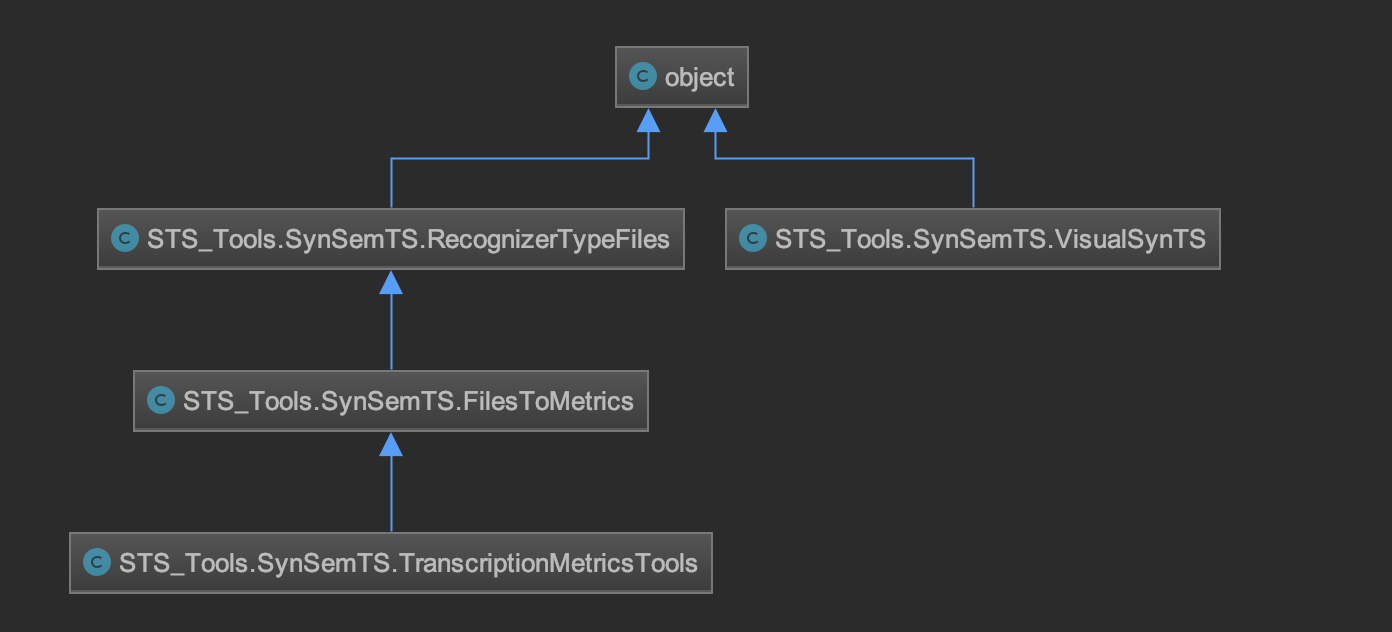
\includegraphics[width=14cm]{images_partie_3/uml_synsemts.png}}}
    \caption{Diagramme du module \citecode{SynSemTS.py} présentant les différentes classes \textcopyright L. Terriel, 2020, \textit{Pycharm}}
    \label{fig:diag_synsem}
\end{figure}

En reprenant le diagramme, une première classe (\citecode{RecognizerTypeFiles}) permet d'identifier les différents types de fichiers correspondant à la transcription vérité terrain, à la prédiction, à l'image et permet également d'effectuer certains traitements textuels sur les fichiers texte, comme le découpage en mots et en caractères. 

Une seconde classe (\citecode{FilesToMetrics}) qui hérite des propriétés et méthodes de la première, effectue la transition entre la première classe et la troisième, en réalisant les calculs de la distance de Levenshtein et en récupérant les résultats sous forme d'entier et de matrice. Ce résultat permet en outre, d'effectuer les futurs calculs.

Une troisième classe (\citecode{TranscriptionMetricsTools}), la plus importante, hérite de la première et de la deuxième. Elle se charge des dernières tâches de normalisation textuelle (suppression des \textit{stop words}) et réalise les calculs permettant de retrouver les métriques qui seront affichées plus tard dans le navigateur \textit{web} (distance de Hamming, WER, CER, indice de Jaccard et similarité cosinus). Dès lors, les objets créés à la fin du \textit{script} principal \citecode{kraken\_benchmark.py} sont issus de la dernière classe. 

Une autre classe est créée indépendamment (\citecode{VisualSynTS}); elle permet de réaliser des objets spécifiques correspondant aux visualisations graphiques affichées dans le navigateur \textit{web}. En revanche, pour des raisons de temps de chargement trop longs, j'ai décidé de créer ces objets dans les routes (\citecode{routing.py}) au moment où l'utilisatrice ou l'utilisateur formule une requête pour les consulter.\\

Pour conclure, il n'était pas obligatoire de programmer avec ce paradigme, mais les avantages de la programmation orientée objet sont nombreux et ont séduit pour la suite du projet. 

Chaque objet présente une documentation claire quant à ses propriétés et ses méthodes, ce qui permet de savoir quels types de fonctions on manipule pendant le développement. Les types d'objets créés peuvent servir de base pour d'autres objets (on évite ainsi de réécrire du code existant). On peut réutiliser ces objets dans le cadre d'autres projets en réutilisant certaines briques déjà posées dans ces classes. 

Enfin en plus d'obtenir un code plus compréhensible, il est plus facile de le maintenir et de le faire évoluer. On pourra modifier les objets, par exemple, ajouter de nouvelles métriques ou les corriger, sans toucher à l'ensemble de l'interface comme la séquence HTR ou la partie affichage dans le navigateur.

\subsubsection{Retour sur les principales difficultés rencontrées}

Parmi les difficultés auxquelles je me suis heurté au cours du développement de l'application, on peut relever les points suivants :

\begin{itemize}
    \item La gestion des données d'entrée (fichiers texte, images et modèle) n'est pas encore optimale. Actuellement, l'utilisatrice ou l'utilisateur doit stocker ses fichiers à la racine du \textit{script} principal suivant un système d'étiquetage comme on l'a vu plus haut. Ce système pourrait être amélioré;
    \item Durant le développement de la fonction coïncidant avec la séquence HTR, je devais trouver le moyen de stocker et d'associer les fichiers entre-eux sans perdre l'ordre des fichiers pour ne pas mélanger une prédiction avec sa vérité terrain et son image. Je pouvais aboutir à des structures de données trop complexes (liste imbriquées de tuples) à manipuler. Je devais souvent lancer le programme en entier, plusieurs fois, pour être sûr que l'ordre n'avait pas été modifié. La programmation objet m'a permis de résoudre le problème;
    \item N'étant pas familier de la programmation objet au moment de coder l'application, beaucoup d'essais ont étaient nécessaires pour aboutir au résultat actuel. Le module \citecode{SynSemTS.py} doit encore pouvoir être simplifié. Une réflexion doit être menée sur cet aspect qui permettrait d'accélérer davantage le processus de création des objets à la fin du script principal;
    \item Je n'ai pas réussi à trouver le moyen d'afficher deux visualisations graphiques différentes sur la même route URL. 
\end{itemize}

\section{Suivi sur la conception et retour sur les usages de \textit{Kraken-Benchmark}}

\subsection{La gestion du projet \textit{Kraken-Benchmark}}\label{gestion_projet}

Durant le développement de l'application, un ensemble de rituels a été mis en place afin de s'assurer des retours réguliers lors du développement de l'application.\\

\textbf{Revue de code et intégration continue - }Dans un premier temps, afin de vérifier que le code répondait aux exigences des règles d'usages propres au langage Python (obtenir un code \inquote{pythonique}), et qu'il était suffisamment compréhensible, un système d'intégration continue a été rendu accessible sur la plate-forme \textit{GitLab} par Alix Chagué, au moment de mon arrivée\footnote{Dans le cadre de mon stage il s'agissait du logiciel \textit{Jenkins} interfacé avec la plate-forme Gitlab.}. À chaque fois que j'ajoutais une fonctionnalité ou que j'effectuais une modification dans mon code, je le déposais sur \textit{GitLab} par l'intermédiaire du système de versions \textit{Git} : j'indiquais dans un message les modifications effectuées (commande \textit{git commit}) et j'envoyais le code sur la plate-forme (commande \textit{git push}). Au moment où la plate-forme Gitlab recevait le code, le système d'intégration continue exécutait automatiquement un fichier BASH (\citecode{ci-test.sh}\footnote{Ce fichier est disponible dans les Annexes \ref{annexe_KB}}), rédigé par Alix Chagué. \\

Ce fichier réalisait un test sur le code source, par le biais du logiciel \textit{Pylint}, pour effectuer une vérification de qualité. \textit{Pylint} utilise les recommandations officielles de la PEP8\footnote{Les PEP (\textit{Python Enhancement Proposal}), sont connues au sein de la communauté Python pour être des propositions d'améliorations du langage Python qui portent toutes un numéro. La PEP8 peut être vue comme un guide pour rédiger en langage Python et a pour objectif de définir des règles de développement communes entre développeurs : vérifier les indentations du code, les noms de variables, les espaces ou les lignes trop longues; PEP8, URL : \url{https://www.python.org/dev/peps/pep-0008/}} pour s'assurer que les règles de rédaction du code sont respectées. Si le score était supérieur à 7, le système me renvoyait un message de succès. Ma responsable pouvait alors entreprendre une revue \inquote{manuelle} du code (\textit{code review}) et se concentrer sur ses aspects fonctionnels du programme, une fois que j'avais effectué des propositions de modifications (\textit{Merge Requests}). Dans le cas contraire, je devais reprendre mon code et repasser les tests. \\

Ce système, bien qu'en apparence contraignant, m'a obligé à assurer une rigueur tout au long de la rédaction de mon code, au fur et à mesure des développement et m'a permis d'accroître mes réflexes tels que la rédaction d'une documentation pour chaque fonctions, nommage des variables etc.
\newpage
\textbf{Tests fonctionnels et retours utilisateurs - } Sur ce point, les tests fonctionnels ont primés sur la rédaction de tests unitaires. On entend par tests unitaires un ensemble de scripts rédigés en langage Python, qui permettent de tester et de s'assurer du bon fonctionnement de plusieurs parties spécifiques du code.  \textit{Kraken-Benchmark} est considéré comme une application \inquote{non-critique} et qui fait une large part à l'expérimentation ; elle est actuellement utilisée par un nombre restreint de personnes au sein d'ALMAnaCH. Une fonctionnalité défaillante n'entraîne donc pas de retard conséquent pour l'avancement du projet, contrairement à une application comme \textit{eScriptorium}, par exemple, qui doit être opérationnelle pour un grand nombres d'usages. 

De plus, les difficultés rencontrées pour développer certaines fonctionnalités essentielles de l'application, conjuguées au besoin de pouvoir effectuer des tests sur des données Lectaurep avant la fin du stage, m'ont obligé à me concentrer sur l'aspect général et les résultats visibles de l'application, plutôt que de couvrir, par la rédaction de tests longs, chaque détails de fonctionnement de l'application.

Cependant, si l'outil doit évoluer dans la suite du projet, ou inclure de nouvelles fonctionnalités et hypothétiquement être mis en production à plus grande échelle, la rédaction de tests unitaires s'avérera être une priorité absolue afin s'assurer des bases plus solides.\\

Pour être sûr que l'application fonctionnait à chaque modification importante, je la relançait avec mon \textit{set} de test (dossier \citecode{jules\_verne\_set\_test}). Je pouvais ainsi m'assurer que le code fonctionnait toujours et qu'aucun conflit majeur n'était apparu.\\

Enfin j'ai créé une \inquote{zone de test}, sous la forme d'un rapport d'erreurs (\textit{issue}) sur \textit{GitLab} pour recueillir les témoignages d'autres utilisateurs. Ainsi Florianne Chiffoleau, ingénieure en recherche et développement au laboratoire  ALMAnaCH, a eu l'occasion de tester les performances de ses modèles de transcription dans \textit{Kraken-Benchmark} afin de pouvoir les départager, dans le cadre du projet DAHN/MESRI traitant de la correspondance de Paul d'Estournelles de Constant (1852-1924).\\

Ces retours positifs montrent que l'utilisation de l'application peut être généralisée à d'autres projets d'HTR que Lectaurep.\\
\newpage
\subsection{Un tour d'horizon de l'interface \textit{Kraken-Benchmark} et des fonctionnalités actuelles}\label{inter_fonc}
Nous proposons dans cette partie de passer en revue les fonctionnalités implémentées actuellement dans Lectaurep et la manière dont on peut interpréter les résultats.

\textbf{La page d'accueil : tableau général de métriques et visualisation par images (Figure \ref{fig:accueil_KB_1} et Figure \ref{fig:accueil_KB_2}) - } La page d'accueil est la première page rencontrée par l'utilisatrice ou l'utilisateur. Un tableau de métriques (\textit{Dashboard}) permet d'obtenir rapidement des scores sur l'ensemble de son corpus (Figure \ref{fig:accueil_KB_1}). Ces métriques ont été présentées en section \ref{metriques} de ce mémoire. On peut attirer l'attention sur la distance de Hamming. C'est l'indicateur qui permet de révéler rapidement à l'utilisateur si la taille de la vérité terrain et de la prédiction font la même longueur. Dans le cas contraire, un symbole \inquote{$\emptyset$} l'indiquera. Un code couleur renseigne les meilleurs scores obtenus (vert) et les scores moins bons (rouge). De plus, sur la suggestion d'Alix Chagué, des hyperliens placés sur les numéros des images permettent d'accéder à l'image en question avec un niveau de détails plus important (Cf. Figure \ref{fig:accueil_KB_2}). 
À l'échelle de l'image, certaines métriques du tableau sont répétées afin d'éviter des alternances à l'utilisateur entre le haut et le bas de la page.

Un premier graphique montre le nombre de caractères exactement reconnus, supprimés et insérés. Enfin, il est possible d'accéder aux autres fonctionnalités qui montrent d'autres vues de l'application.
\begin{figure}[H]
    \centering
    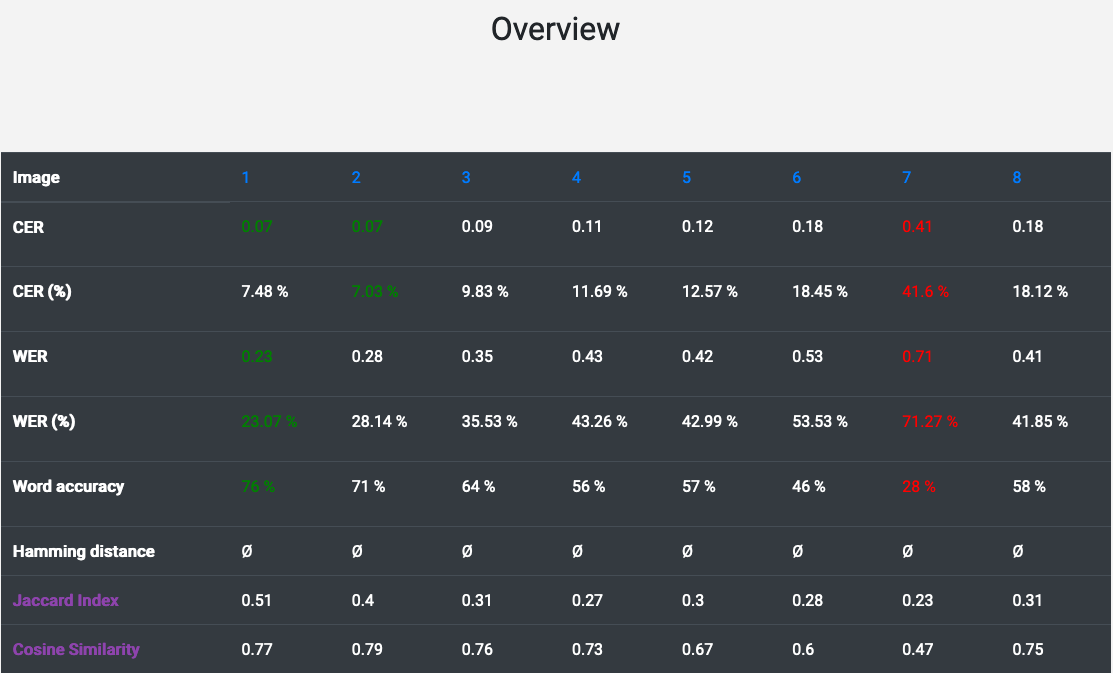
\includegraphics[width=16cm]{images_partie_3/interface_KB/KB_2.png}
        \caption{La page d'accueil : tableau de métriques \textcopyright L.TERRIEL, 2020, \textit{Kraken-Benchmark}}
        \label{fig:accueil_KB_1}
\end{figure}

\begin{figure}[H]
    \centering
    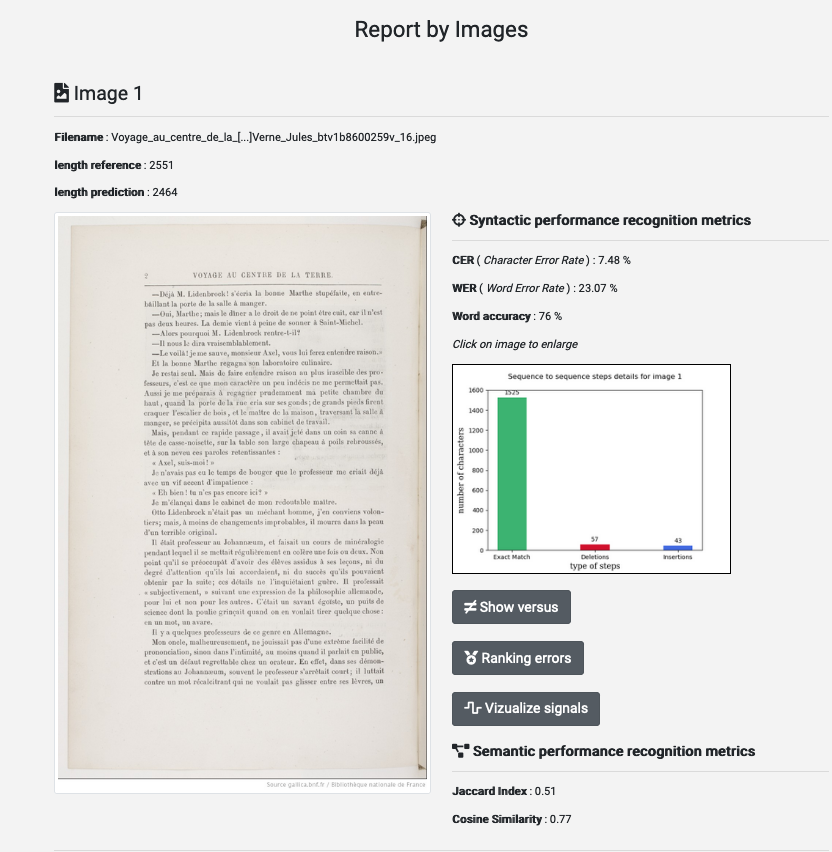
\includegraphics[width=18cm]{images_partie_3/interface_KB/KB_4.png}
        \caption{La page d'accueil : l'image et le graphique des opérations \textcopyright L.TERRIEL, 2020, \textit{Kraken-Benchmark}}
        \label{fig:accueil_KB_2}
\end{figure}
\newpage
\textbf{Une option pour confronter la vérité terrain et la prédiction HTR (Figure \ref{fig:accueil_KB_3}) - } La fonctionnalité \textit{Show versus} de la page d'accueil permet de confronter la vérité terrain dans la colonne de gauche à la prédiction située dans la colonne de droite. La colonne du milieu est une superposition des deux textes. Un code couleur signale à l'utilisatrice ou à l'utilisateur les caractères parfaitement reconnus en vert, les caractères supprimés ou substitués en rouge, et les insertions en bleu. 

Au niveau supérieur, la distance de Levensthein indique à l'utilisateur la mesure des différences entre les deux textes : si le score est supérieur à 10, il s'affiche en rouge pour indiquer que le texte contient un grand nombre d'erreurs.
\begin{figure}[H]
    \centering
    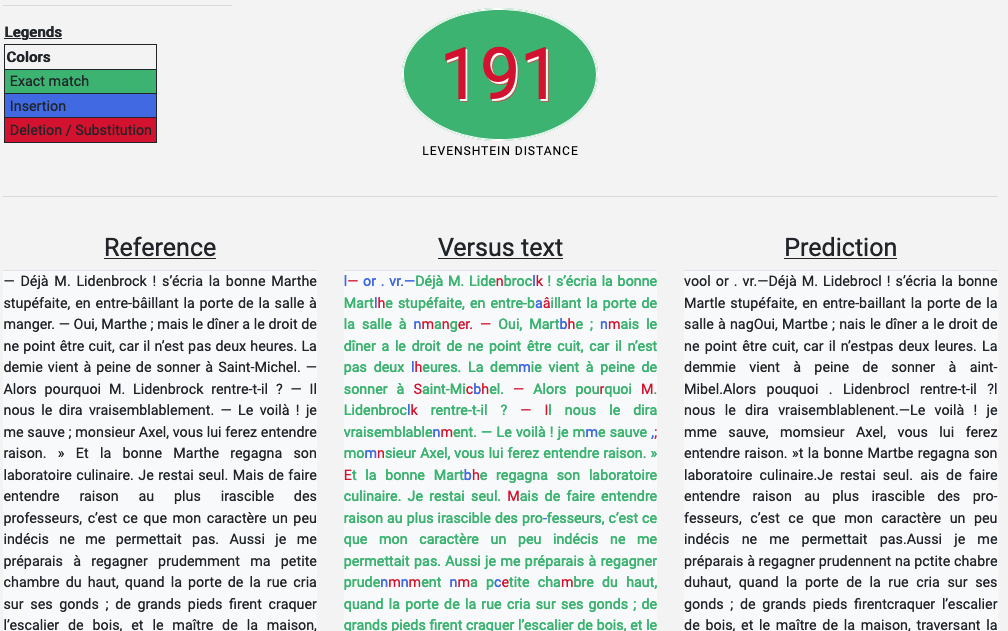
\includegraphics[width=18cm]{images_partie_3/interface_KB/KB_5_VS.png}
        \caption{La fonctionnalité \textit{Show versus} \textcopyright L.TERRIEL, 2020, \textit{Kraken-Benchmark}}
        \label{fig:accueil_KB_3}
\end{figure}
\bigskip

\textbf{Un classement des erreurs les plus fréquentes (Figure \ref{fig:accueil_KB_4}) - }  La fonctionnalité \textit{Ranking errors} est un classement des erreurs les plus fréquentes commises par le modèle sur l'image. L'utilisatrice ou l'utilisateur dispose d'une indication sur la fréquence d'apparition de l'erreur et des détails sur le caractère de la vérité terrain qui a été confondue par le modèle. L'absence de caractère indique un \inquote{espace}. Sur la droite, l'utilisateur dispose d'une autre vue sous la forme d'une \inquote{matrice de confusion}. Il ne s'agit pas d'une \inquote{matrice de confusion} au sens strict, c'est-à-dire une classification des données par classes, il s'agit là du même classement des paires d'erreurs, uniquement pour les dix erreurs les plus fréquentes (sinon la matrice devient illisible). \newpage Ainsi en ordonnée sont disposés les caractères du texte de référence et en abscisses les caractères de la phrase prédite. L'alignement d'un caractère $x$ et d'un caractère $y$ nous donne la fréquence de la confusion. Le classement détaillé à gauche et la matrice à droite, sont équivalentes. 
\begin{figure}[H]
    \centering
    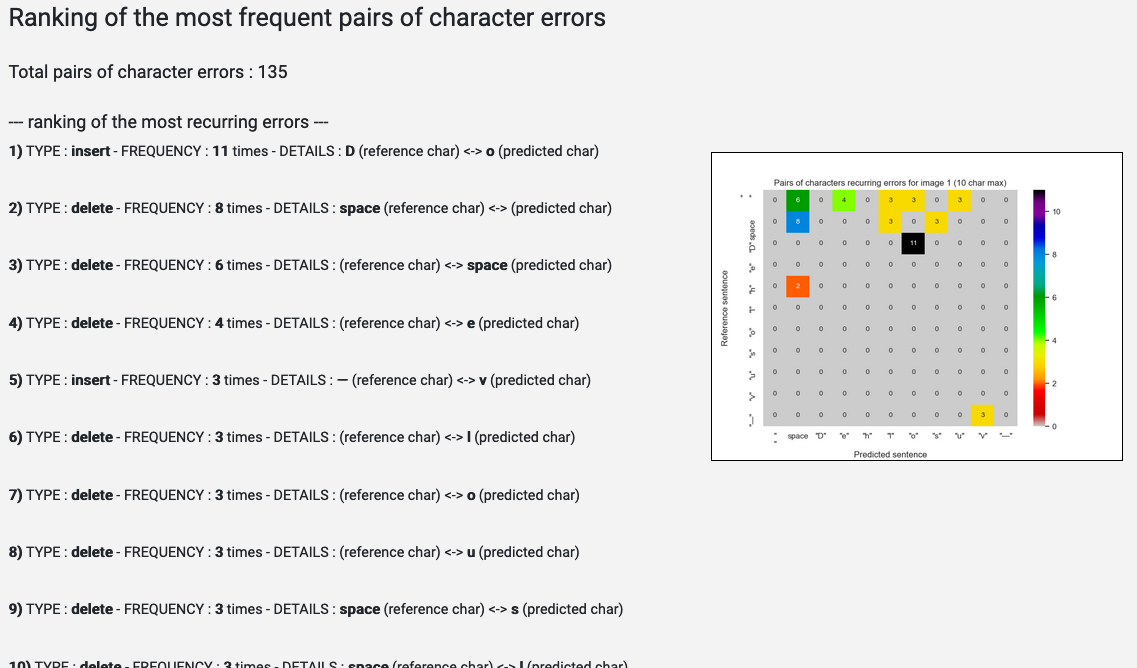
\includegraphics[width=18cm]{images_partie_3/interface_KB/KB_6_rank.png}
        \caption{La fonctionnalité \textit{Ranking errors} \textcopyright L.TERRIEL, 2020, \textit{Kraken-Benchmark}}
        \label{fig:accueil_KB_4}
\end{figure}
\bigskip

\textbf{Une visualisation des phrases sous la forme de signaux (Figures \ref{fig:accueil_KB_5},  \ref{fig:accueil_KB_6} et \ref{fig:accueil_KB_7}) - } La fonctionnalité \textit{Vizualize signals} (Cf. Figure \ref{fig:accueil_KB_5}) permet de générer une visualisation expérimentale qui appartient au module \citecode{STSig.py}\footnote{Le détail de l'algorithme est présenté dans le \textit{notebook} Jupyter intitulé \inquote{Evaluation de la similarité entre deux séquences dans le contexte de la reconnaissance automatique de caractères}.}. 
J'ai essayé de superposer sous la forme de droites le texte de référence et la prédiction. Ces droites passent par des points dont les coordonnées correspondent, en abscisses, à l'ordre d'enchaînement des caractères dans les deux textes, et, en ordonnées, des valeurs numériques correspondant aux caractères, eux-mêmes accessibles par l'onglet \textit{Dictionnary position-weight characters}. Il s'agit d'un dictionnaire qui permet de décoder les valeurs numériques de l'axe des ordonnées.\\ 

\begin{figure}[h!]
    \centering
    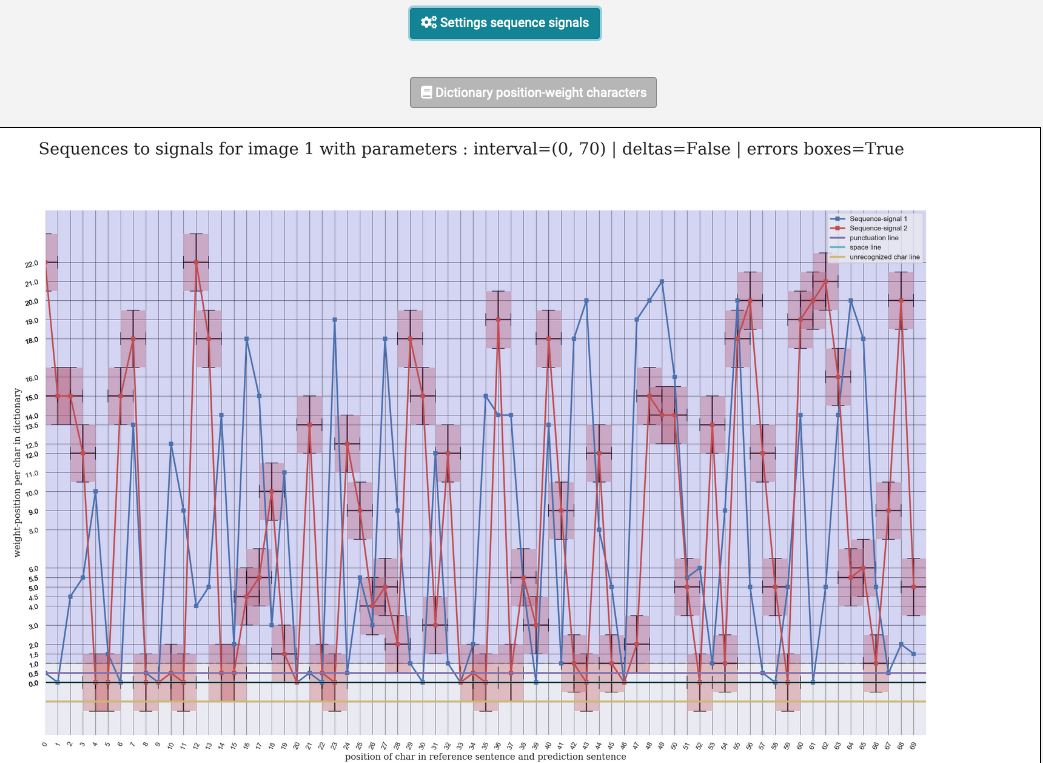
\includegraphics[width=17cm]{images_partie_3/interface_KB/KB_7_STS.png}
        \caption{La fonctionnalité \textit{Vizualize signals} \textcopyright L.TERRIEL, 2020, \textit{Kraken-Benchmark}}
        \label{fig:accueil_KB_5}
\end{figure}
\newpage
Ces valeurs numériques en ordonnées sont construites selon un système de pondération comme suit : un caractère de ponctuation sera associé à une pondération de 0.5, un espace à 0, et un caractère non reconnu ou des chiffres à une valeur de -1.

Chaque caractère de l'alphabet latin est encodé de la manière suivante : \inquote{a} vaudra 1, \inquote{b} vaudra 2, \inquote{c} vaudra 3 etc. 
Si ces caractères subissent une ou des transformation(s) on leur ajoute un poids : une accentuation vaudra 0.5, une capitalisation 0.1 et une capitalisation ajoutée à une accentuation 0.6. Par exemple si \inquote{a} vaut 1 alors \inquote{à} vaudra 1.5 et un \inquote{À} vaudra 1.6, de même si \inquote{b} vaut 2 alors \inquote{B} vaudra 2.1 etc.
Dès lors, l'algorithme encode la vérité terrain et la prédiction selon ce système de valeurs numériques. L'algorithme récupère les coordonnées, pour représenter les deux textes sous la forme de droites. 
Si les deux droites se confondent, cela signifie que la prédiction correspond à la référence. Cependant si un caractère de la prédiction diffère de celui de la référence, une structure en boîtes d'erreurs (\textit{error boxes}, représentées comme des boîtes rouges sur la figure \ref{fig:accueil_KB_5}) se met en place sur les points représentants les caractères de la prédiction divergeant de la référence. On peut alors interpréter certains phénomènes sur le graphique pour comprendre les erreurs récurrentes (Cf. Figure \ref{fig:accueil_KB_7}).\\

\begin{figure}[h!]
    \centering
    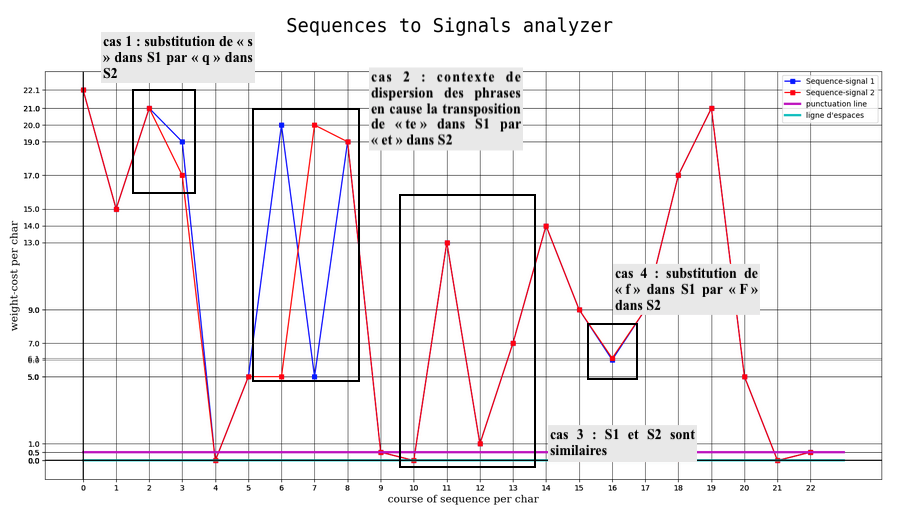
\includegraphics[width=15cm]{images_partie_3/interface_KB/graph_sequence_signal.png}
        \caption{Exemples d'interprétations de la fonctionnalité  \textit{Vizualize signals} \textcopyright L.TERRIEL, 2020, \textit{Kraken-Benchmark}}
        \label{fig:accueil_KB_7}
\end{figure}

Dans le but de ne pas surcharger le graphique et prendre le risque de le rendre illisible, un système d'intervalles est réglable (Cf. Figure \ref{fig:accueil_KB_6}) par l'utilisatrice ou l'utilisateur pour accéder à certaines parties des textes par le biais de l'onglet \textit{Settings sequence signals}. Cette représentation est un essai, et elle ne peut se substituer aux métriques classiques d'évaluation des modèles HTR présentées plus haut; de plus un trop grand nombre d'erreurs rend rapidement la lecture impossible.

\begin{figure}[h!]
    \centering
    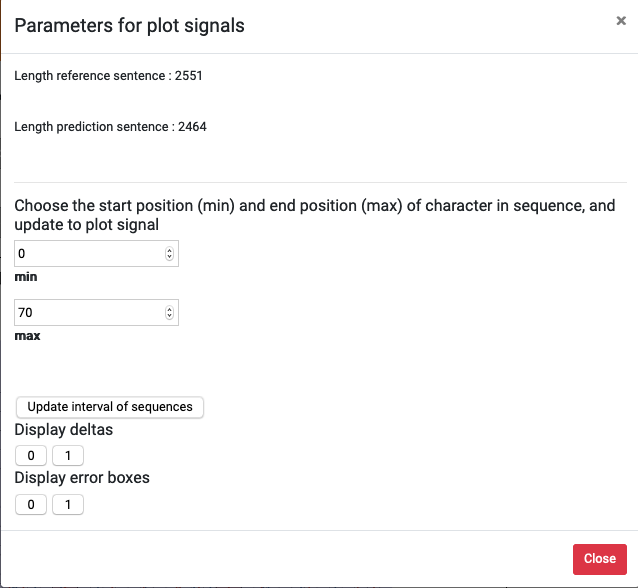
\includegraphics[width=9cm]{images_partie_3/interface_KB/KB_8_STS.png}
        \caption{La fenêtre \inquote{pop-up} qui permet de régler l'intervalle des séquences à visualiser dans le graphique de \textit{Vizualize signals} \textcopyright L.TERRIEL, 2020, \textit{Kraken-Benchmark}}
        \label{fig:accueil_KB_6}
\end{figure}

\newpage
\section{Perspectives d'amélioration techniques pour l'application}\label{perspectives_amélios}

Dans la section \ref{objectifs}, nous avions fixé plusieurs objectifs à atteindre. À la fin du stage, certaines de ces tâches ont été réalisées et d'autres non pas pu l'être dans les temps. 

L'outil proposé actuellement est opérationnel pour tester des modèles de transcription, regroupant les métriques classiques d'évaluation de l'HTR. Cependant, l'outil peut encore être largement amélioré, voici un potentiel cahier des charges de l'application :
\begin{itemize}
    \item Dans la section \ref{gestion_projet}, nous avons évoqué le manque de tests unitaires pour l'application;
    \item La gestion des données en entrée peut bénéficier d'améliorations conséquences : possibilité pour l'utilisatrice ou l'utilisateur de choisir un chemin sans avoir à trier ses données en amont du projet et de les étiqueter par un système de label dans le nommage des fichiers, le programme associant automatiquement la bonne image à sa transcription de vérité terrain. De plus, l'utilisatrice ou l'utilisateur doit pouvoir importer ses données dans des formats structurés comme le XML-TEI;
    \item La seule manière de conserver le rapport est de sauvegarder la page HTML : l'application devrait proposer l'export du rapport dans des formats structurés comme XML-TEI ou XML ALTO ou encore en PDF. Le XML ALTO permet d'inclure des métriques comme le taux de confiance de reconnaissance (\textit{word accuracy}) dans des éléments prédéfinis; 
    \item Un scénario envisageable pourrai faire correspondre le fichier XML-TEI en import et en export dans l'application au format pivot XML-TEI de Lectaurep présenté dans la partie \ref{partie_2} (Cf. Figure \ref{fig:TEI-KB})
    \item Certaines étapes de la séquence du traitement HTR dans l'application devraient être optionnelles (la binarisation par exemple);
    \item D'autres traitements TAL pourraient être proposés dans \textit{Kraken-Benchmark}, ainsi l'application pourrait être interfacée avec l'API d'\textit{Entity-Fishing} et paramétrée avec le référentiel souhaité pour tester les modèles spécifiquement entraînés à la reconnaissance d'entités nommées; 
    \item Actuellement, il n'est pas possible d'utiliser son propre modèle de segmentation dans l'application. À noter qu'au début du stage la documentation de l'API Kraken était moins fournie, ce qui n'est plus le cas;
    \item Découlant de la proposition précédente, l'évaluation des modèles de segmentation dans l'application n'a pas été implémentée. Cependant la documentation de l'API Kraken enrichie depuis peu, ainsi qu'une rapide prospection des outils dans les dépôts de code montrent que cela est réalisable\footnote{Le code du dépôt \textit{TMG\_ImageAnnotation} disponible sur GitHub propose un module d'annotation d'images qui pourrait être adapté pour les besoins d'évaluation de la segmentation pour \textit{Kraken-Benchmark}. En combinaison avec les fonctions de l'API Kraken et le \textit{package} Python \textit{PIL} pour le traitement d'images; on pourrait implémenter dans \textit{Kraken-Benchmark} une visualisation de la segmentation sous la forme de rectangles entourant les zones de textes sur l'image indiquant si la segmentation a été correctement effectuée, via un code couleur, sur les images. \textit{TMG\_ImageAnnotation}, URL : \url{https://github.com/guillotel-nothmann/imageAnnotation}};
    \item La partie CLI, qui permet le chargement des données dans \textit{Kraken-Benchmark}, constitue une solution provisoire. Elle pourrait bénéficier d'une interface graphique au même titre que la partie visualisation de données dans le navigateur \textit{web}. Cela est possible en migrant le script principal \citecode{kraken\_benchmark.py} vers un système de routes basé sur \textit{Flask} et des \textit{templates} HTML associées pour téléverser les fichiers dans une interface graphique;
    \item Au lieu de se servir de l'actuel serveur de développement du \textit{micro-framework Flask}, le programme pourrait reposer sur un serveur, comme Heroku\footnote{\textit{Heroku - Cloud Application Platfrom}, URL : \url{https://www.heroku.com/}}, pour permettre le déploiement de \textit{Kraken-Benchmark} sur le \textit{web} et sans avoir à lancer l'application depuis le terminal. Dans, une autre optique \textit{Kraken-Benchmark} pourrait constituer une fonctionnalité (\textit{plugin}) intégrée à \textit{eScriptorium}\footnote{\textit{eScriptorium} est programmé avec le \textit{framework Django} qui, comme \textit{Flask}, repose sur une architecture de type MVT (Modèle-Vue-\textit{Templates}) dès lors une migration vers ce projet doit être réalisable.}. Ainsi l'utilisatrice ou l'utilisateur effectuant ses vérités terrains et l'entraînement de ses modèles sur \textit{eScriptorium} pourrait jouïr d'un relais vers \textit{Kraken-Benchmark} pour mesurer l'efficacité de son modèle. Ce dernier point nécessite cependant d'avoir répondu à l'ensemble des tâches précédentes.
\end{itemize}

\begin{figure}[h!]
    \centering
    \centerline{\fbox{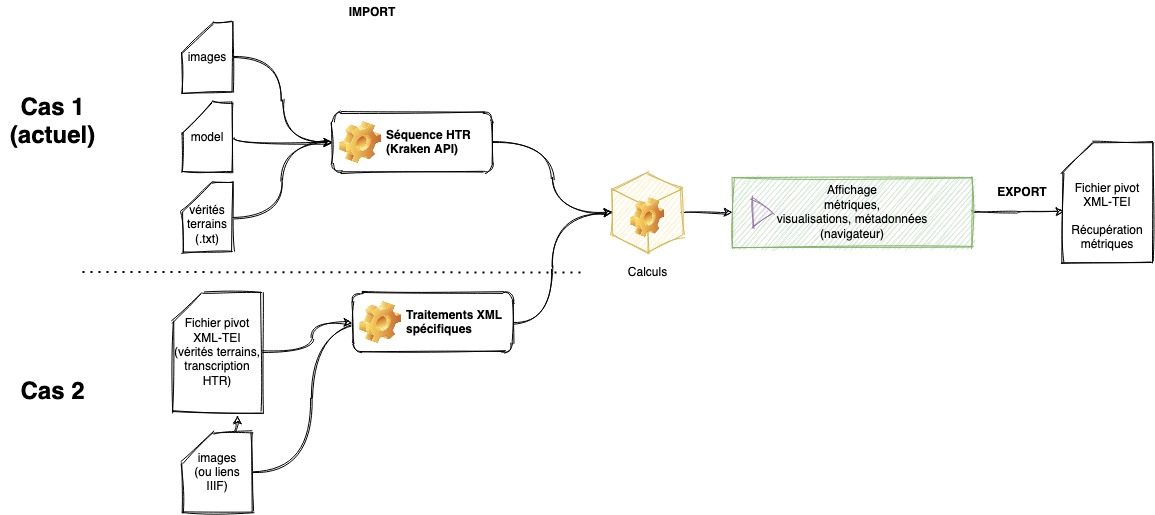
\includegraphics[width=19cm]{images_partie_3/scenari_KB.png}}}
    \caption{Le Cas 2 représente un scénario utilisateur envisageable dans \textit{Kraken-Benchmark} \textcopyright L. Terrie, 2020, \textit{Diagrams.net}}
    \label{fig:TEI-KB}
\end{figure}

\thispagestyle{empty}
\chapter{Tests de \textit{Kraken-Benchmark} sur les données Lectaurep}\label{tests_KB_lectaurep}

Au moment où \textit{Kraken-Benchmark} a atteint une version \inquote{stable}, j'ai envisagé d'expérimenter l'outil avec des données Lectaurep pour évaluer les modèles HTR et de simuler des usages répétitifs de l'outil en vue de la suite du projet\footnote{Pour davantage de détail consulter le compte-rendu en Annexes \ref{annexe_KB}, \citecode{CR\_tests\_lectaurep\_KB.md}. De plus l'ensemble des fichiers présenté ci-dessous sont disponibles en Annexes \ref{annexe_KB}, \citecode{sets\_tests\_lectaurep/}}.

\section{Préparation des jeux de données} 

\subsection{Les images} 
Durant le stage il a été convenu de tester l'outil sur des images \inquote{extrêmes}, c'est-à-dire présentant des particularités d'écritures remarquables et des images de répertoire présentant des défauts physiques ou de numérisation. Aurélia Rostaing, responsable du pôle des instruments de recherche et coordinatrice du projet Lectaurep, ainsi que les annotatrices et les annotateurs du DMC sur la plate-forme d'\textit{eScriptorium} ont effectué un travail de repérage important pour relever des images présentant des particularismes. A la réception du corpus d'images, j'ai constitué quatre jeux de données, composé chacun de trois images :

\begin{itemize}
    \item \textit{Set\_material\_defects} : jeu contenant des images présentant des défauts matériels ou des défauts de numérisation (Cf. Figure \ref{fig:exemples_material});
    \item \textit{Set\_writing\_defects} : jeu composé d'images de répertoires comportant des éléments de graphies atypiques (typographies, signes et symboles) (Cf. Figure \ref{fig:exemples_write});
\end{itemize}
\newpage
\begin{figure}[H]
    \begin{minipage}[c]{.46\linewidth} 
        \centering
        \textbf{1)}
        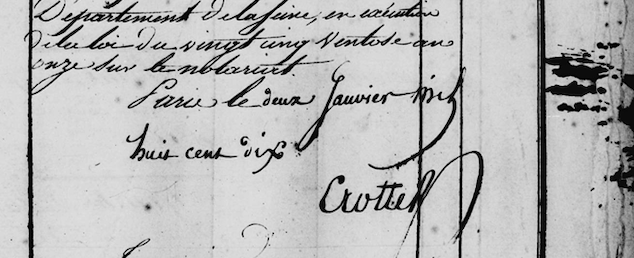
\includegraphics[width=8cm,height=7cm]{images_partie_3/particularismes/material_1.png}
        \end{minipage}
    \hfill%
    \begin{minipage}[c]{.46\linewidth}
        \centering
        \textbf{2)}
        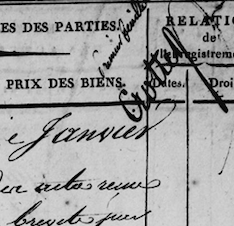
\includegraphics[width=8cm,height=7cm]{images_partie_3/particularismes/material_2.png}
    \end{minipage}
    \hfill%
    \begin{minipage}[c]{.46\linewidth}
        \centering
        \textbf{3)}
        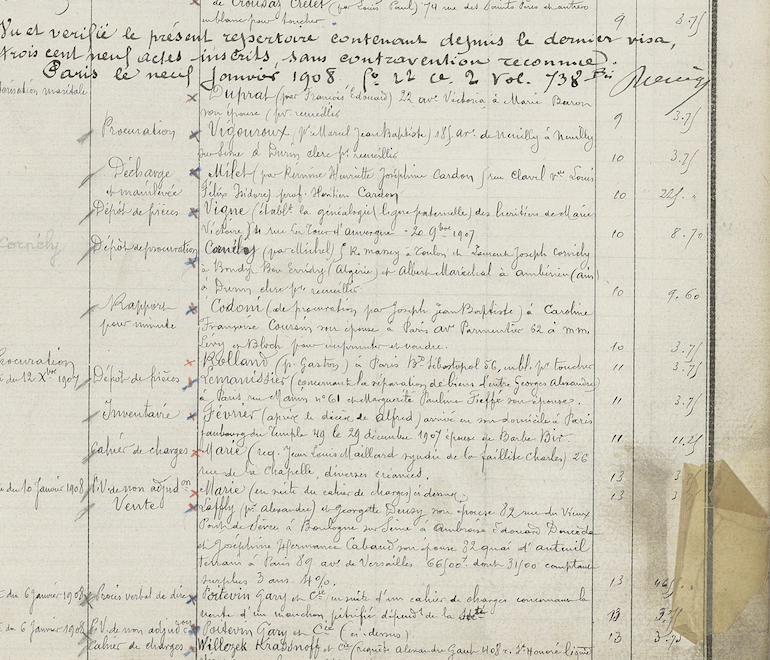
\includegraphics[width=8cm,height=7cm]{images_partie_3/particularismes/material_3.png}
    \end{minipage}
    \hfill%
    \begin{minipage}[c]{.46\linewidth}
        \centering
        \textbf{4)}
        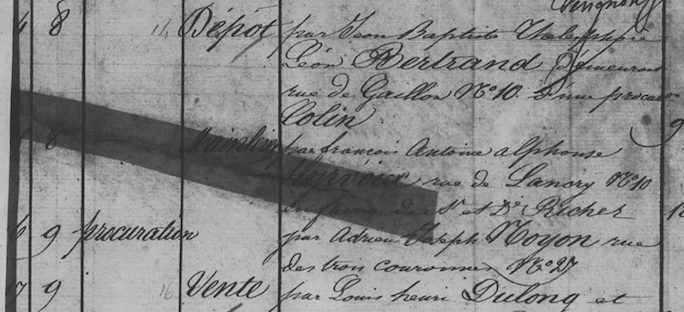
\includegraphics[width=8cm,height=7cm]{images_partie_3/particularismes/material_4.png}
    \end{minipage}
        \caption{\textit{Set\_material\_defects} : les focus 1) et 2) correspondent à l'image \citecode{subject\_1\_robin\_DAFANCH96\_048MIC04695\_L-1.jpeg}, (N\&B, étude XLVIII, notaire Jean-François Robin), présentant des tâches d'encre et des écritures marginales, des noirceurs et des forts contrastes; le focus 3) 
        \citecode{subject\_2\_rigault\_FRAN\_0187\_16416\_L-1.jpeg}, (couleurs, étude LXXXVI, notaire Jean-Paul Rigault), 
        présentant un ruban adhésif sur la partie inférieure droite du document obstruant une partie des colonnes 6 et 7; le focus 4)
        \citecode{subject\_3\_michaux\_DAFANCH96\_MIC067000672-1.jpeg}, (N\&B, étude VII, Pierre Michaux) présentant un ruban adhésif épais obstruant une partie du texte dans les colonnes 1, 2, 3, et 4 et une très mauvaise qualité de numérisation.
        \textcopyright AN-DMC, 2020}
    \label{fig:exemples_material}
\end{figure}

\newpage
\begin{figure}[H]
    \begin{minipage}[c]{.46\linewidth} 
        \centering
        \textbf{1)}
        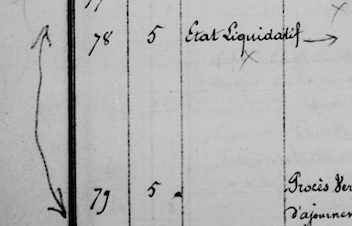
\includegraphics[width=8cm,height=7cm]{images_partie_3/particularismes/write_1.png}
        \end{minipage}
    \hfill%
    \begin{minipage}[c]{.46\linewidth}
        \centering
        \textbf{2)}
        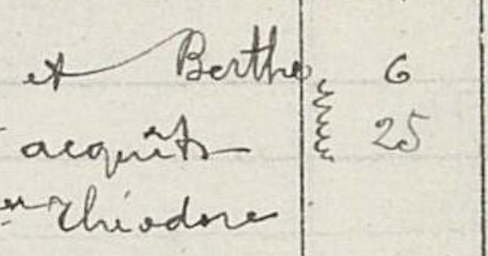
\includegraphics[width=8cm,height=7cm]{images_partie_3/particularismes/write_2.png}
    \end{minipage}
    \hfill%
    \begin{minipage}[c]{.46\linewidth}
        \centering
        \textbf{3)}
        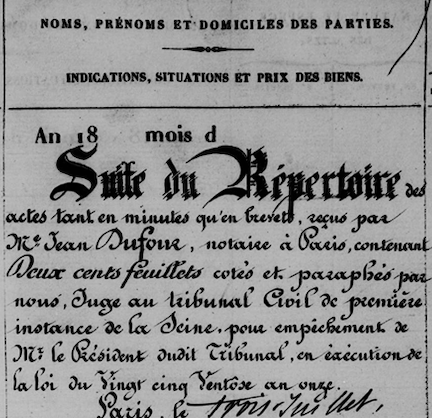
\includegraphics[width=8cm,height=7cm]{images_partie_3/particularismes/write_3.png}
    \end{minipage}
        \caption{\textit{Set\_writing\_defects} : le focus 1) correspond à l'image \citecode{subject\_1\_dufour\_DAFANCH96\_048MIC07685\_L-0.jpeg}, (N\&B, étude XLVIII, notaire Jean Dufour), présentant une double flèche dans le coin inférieur gauche du répertoire au niveau de la colonne 1 ; le focus 2) correspond à l'image \citecode{subject\_2\_rigault\_FRAN\_0187\_16428\_L-1.jpeg}, (N\&B, étude LXXXVI, notaire Jean-Paul Rigault),  présentant un élément atypique situé au niveau du nombre \inquote{25} de la colonne 6 correspondant aux \inquote{dates}; le focus 3) correspond à l'image
        \citecode{subject\_3\_dufour\_DAFANCH96\_048MIC08733\_L-1.jpeg}, (N\&B, étude XLVIII, notaire Jean Dufour) présentant une calligraphie fracturée.
        \textcopyright AN/DMC, 2020}
    \label{fig:exemples_write}
\end{figure}
\newpage    
Viennent ensuite deux \textit{sets} témoins pour compléter l'expérience et comparer les résultats :

\begin{itemize}
    \item \textit{homogeneous\_control\_set} : comportant des images n'ayant subit aucune interférence lors de la numérisation du corpus et présentant des graphies régulières, une présentation des écritures réparties dans les colonnes du tableau de manière homogène, sans altération matérielle apparente des répertoires de notaire, provenant de la même étude XLIII du notaire Louis Marie Joseph Marotte; 
    \item \textit{different\_control\_set} : similaire aux caractéristiques du premier jeu de données présenté ci-dessus, à la différence près que les images proviennent chacune d'une autre étude. 
\end{itemize}

\subsection{Les modèles} 
Les modèles utilisés pour le test ont été entraînés par Alix Chagué et Floriane Chiffoleau à ALmanaCH, par le système HTR :

\begin{itemize}
    \item \citecode{model\_test\_lectaurep\_bin\_accuracy\_6064.mlmodel} : a été entraîné avec 135 pages du notaire Rigault et sur 23 \textit{epochs}. Il s'agit du modèle de l'époque 18 avec un \textit{accuracy} de 0.6064.\footnote{Lectaurep disposait encore de trop peu de vérités terrains, de plus il y a eu des problèmes de compatibilité entre le serveur RIOC (\textit{cluster} de calcul) et les dépendances de Kraken.}  
    \item \citecode{model\_test\_lectaurep\_bin\_accuracy\_8164.mlmodel} : a été entraîné au début du projet Lectaurep avec 67 pages du notaire Marotte et sur 14 \textit{epochs}. Il s'agit du modèle de l'époque 9 avec un \textit{accuracy} de 0.8164.
\end{itemize}

\subsection{Les vérités terrains}

Pour les deux \textit{sets} présentant des particularismes, les vérités terrains ont été réalisées par Danis Habib, chargé d'études documentaires au DMC, sur la plate-forme \textit{eScriptorium}. Elles m'ont été transmises dans un format texte.

Pour les \textit{sets} témoins, les vérités terrains étaient disponibles sur la plate-forme \textit{Sharedocs} au format XML ALTO. J'ai donc récupéré un script Python de la Bibliothèque d'État de Berlin\footnote{Ce script est disponible dans les Annexes \ref{annexe_KB}, \citecode{alto2text.py}} qui permet la conversion du XML ALTO vers un format texte pour retrouver les vérités terrains compatibles avec \textit{Kraken-Benchmark}. 
\newpage
\section{Méthodologie et résultats obtenus}

Pour effectuer les tests j'ai passé successivement chacun des jeux de données, présentés plus haut, contenant les documents de vérité terrains, les images avec les deux modèles dans l'outil \textit{Kraken-Benchmark}. J'ai établi un compte rendu (\citecode{CR\_tests\_lectaurep\_KB.md}) dans lequel j'ai relevé l'ensemble des métriques obtenues et effectué des sauvegardes de la page HTML de la fonctionnalité \textit{versus-text} de l'application qui permet la confrontation de la vérité terrain et de la prédiction\footnote{Ces captures sont disponibles dans les Annexes \ref{annexe_KB}, \citecode{snaps\_tests\_lectaurep/}}.

J'ai ensuite collecté spécifiquement les résultats WER, CER et le taux de reconnaissance par mot dans deux tableurs CSV\footnote{Ces tableurs sont disponibles dans les Annexes \ref{annexe_KB}, \citecode{details\_data\_average\_tests\_model\_test\_lectaurep\_\\bin\_accuracy\_6064.mlmodel- Feuille 1.pdf} et \citecode{details\_data\_average\_tests\_model\_test\_lectaurep\_\\bin\_accuracy\_8164.mlmodel- Feuille 1.pdf}} (\textit{Comma Separated Values}) et réaliser des moyennes globales pour chaque jeu de données à partir de ces taux. Ils sont reportés dans les deux tableaux ci-dessous :
\bigskip

\begin{tabular}{|1|l|l|l|}
  \hline
  \multicolumn{4}{|c|}{Résultats modèle \textit{lectaurep\_bin\_accuracy\_6064}} \\
  \hline & Moyenne CER & Moyenne WER & Moyenne \textit{Word Accuracy}* \\ 
  \hline homogeneous\_control\_set & 76.78 \% & 94.64 \% & 5 \% \\
  \hline different\_control\_set & 72.30 \% & 93.0 \% & 7 \% \\
  \hline Set\_writing\_defects & 74.20 \% & 94.50 \% & 4 \% \\
  \hline Set\_material\_defects & 75.36 \% & 96.15 \% & 3 \% \\
  \hline
\end{tabular}
\bigskip

\begin{tabular}{|1|l|l|l|}
  \hline
  \multicolumn{4}{|c|}{Résultats modèle \textit{lectaurep\_bin\_accuracy\_8164}} \\
  \hline & Moyenne CER & Moyenne WER & Moyenne \textit{Word Accuracy}* \\ 
  \hline homogeneous\_control\_set & 70.0 \% & 96.16 \% & 4 \% \\
  \hline different\_control\_set & 69.21 \% & 93.62 \% & 6 \% \\
  \hline Set\_writing\_defects & 73.0 \% & 96.70 \% & 3 \% \\
  \hline Set\_material\_defects & 73.0 \% & 97.46 \% & 2 \% \\
  \hline
\end{tabular}
\begin{center}
    \small{* \textit{mesure arrondie à l'entier}}
\end{center}

\bigskip

Les résultats de ces deux séries de tests sont globalement mauvais quant aux perspectives de récupération d'une transcription propre et lisible avec ces modèles. 

Si l'on observe les deux tableaux ci-dessus les moyennes du WER et du CER sont élevés : généralement entre 70\% et 100\%. Le taux de reconnaissance par mots (\textit{word accuracy}) lui ne dépasse pas la barre des 10\%. Le modèle commet des fautes sur l'ensemble des mots du texte. De plus, on remarque que les résultats sont à la fois très faibles et en même temps très proches dans le cas des deux modèles.\\

Durant les tests, certaines visualisations qu'offre \textit{Kraken-Benchmark} n'ont pas pu être utilisées (classement des paires d'erreurs, et visualisations en signaux). En cause, le nombre important d'insertions et de suppressions élevés dans la prédiction (comme en témoigne les absences de distance de Hamming et les distances d'édition importantes). Le bruit trop intense dans la prédiction provoque des décalages trop importants entre les séquences de caractères correspondant à la référence et à la prédiction. Seul le \textit{dashboard} de métriques et la confrontation à l'oeil nu de la référence et de la prédiction avec l'option \textit{versus text} ont pu être utilisés. 

\section{Un bilan mitigé pour les tests dans\\ \textit{Kraken-Benchmark}?}

Si l'on regarde les taux obtenus par les modèles HTR les plus performants dans d'autres projets, ils restent inférieurs à 20\% et peuvent être considérés comme lisible pour l'oeil humain\footnote{\cite{barrere_results_2018};  \cite{pratikakis_icfhr_2018}; \cite{olver_machine_2017}; \cite{ares_oliveira_comparing_2018} et \cite{lavrenko_holistic_2004}}, en revanche des taux supérieurs à 70\%, comme dans le cas des tests effectués ici, sont non seulement illisibles à l'oeil nu mais aussi moins précis pour un traitement informatique. 

De plus comme l'avait noté Marie-Laurence Bonhomme lors de la phase préliminaire du projet : \inquote{On considère aujourd'hui comme bon un modèle d'HTR qui produit des résultats où le CER est inférieur à 10\%, et comme très bons ceux dont le CER est autour
de 5\%.}\footnote{\cite{bonhomme_defis_2018}, pp.7}. Dès lors, les modèles de transcription utilisés sont bien en deça des attentes de Lectaurep. Plusieurs pistes d'explication sont possibles :
\newpage

\begin{itemize}
    \item Lectaurep n'est pas encore entré dans sa phase de transcription ; nous ne disposions pour ces tests que de très peu de données d'entraînements pour de la reconnaissance d'écriture, comme le modèle sous-ajusté (\textit{underfitted model}) \citecode{model\_test\_lectaurep\_bin\_\\accuracy\_6064.mlmodel} entrainé avec 135 pages. De plus, lors des entraînements de ce modèle, il existait de nombreux conflits entre les dépendances de la version de \textit{Kraken} et l'utilisation du serveur INRIA RIOC.
    \item \textit{Kraken-Benchmark} n'est pas encore capable d'intégrer des modèles de segmentation entraînés spécifiquement pour Lectaurep. L'application utilise actuellement une segmentation par défaut de \textit{Kraken}, ce qui peut, en partie, tromper les résultats.
    \item Les modèles utilisés sont centrés généralement sur des notaires précis (Marotte et Rigault), ce qui peut constituer un biais d'entraînement et poser des problèmes lorsque le modèle doit rencontrer d'autres types de mains dans les répertoires.
\end{itemize}

Depuis la fin du stage, ma responsable a pu informer l'ensemble des acteurs de Lectaurep de l'entraînement de nouveaux modèles  avec des données plus nombreuses : un modèle entraîné sur 18 688 lignes, soit 53 pages du notaire Marotte, avec un taux d'exactitude à 87,46\% (proche des taux obtenu avec \textit{Transkribus} lors de la phase 1), et un modèle entraîné sur 18 688 lignes, soit 100 pages du notaire Riant, avec un taux d'exactitude de 74,67 \%, et un modèle du notaire Dufour entraîné sur 14 590 lignes, soit 89 pages du notaire Dufour, avec un taux d'exactitude de 76,46\%.\\ 

Le taux d'exactitude correspond à un taux de performance du modèles produit durant les itérations d'entraînement (on parle de \textit{Best Accuracy} pour décrire le modèle ayant obtenu le meilleur résultat. Le \textit{Last Accuracy} (terme non conventionnel), décrit en Figure \ref{fig:visual_newmodels}, correspond au taux d'exactitude du modèle de la dernière itération). Les résultats sont disponibles en Figure \ref{fig:visual_newmodels}. Alix Chagué a pu observer que \inquote{le modèle qui obtient le plus haut taux d'erreur est aussi celui qui a produit le plus grand nombre d'itérations sur le corpus de vérité terrain le plus petit}, une hypothèse qui reste à vérifier avec des données plus hétérogènes et plus nombreuses. De plus, ces modèles devraient être testés dans \textit{Kraken-Benchmark} lorsque les modèles de segmentation propres à Lectaurep pourront s'interfacer avec l'application.\\

\begin{figure}[H]
    \centering
    \centerline{\fbox{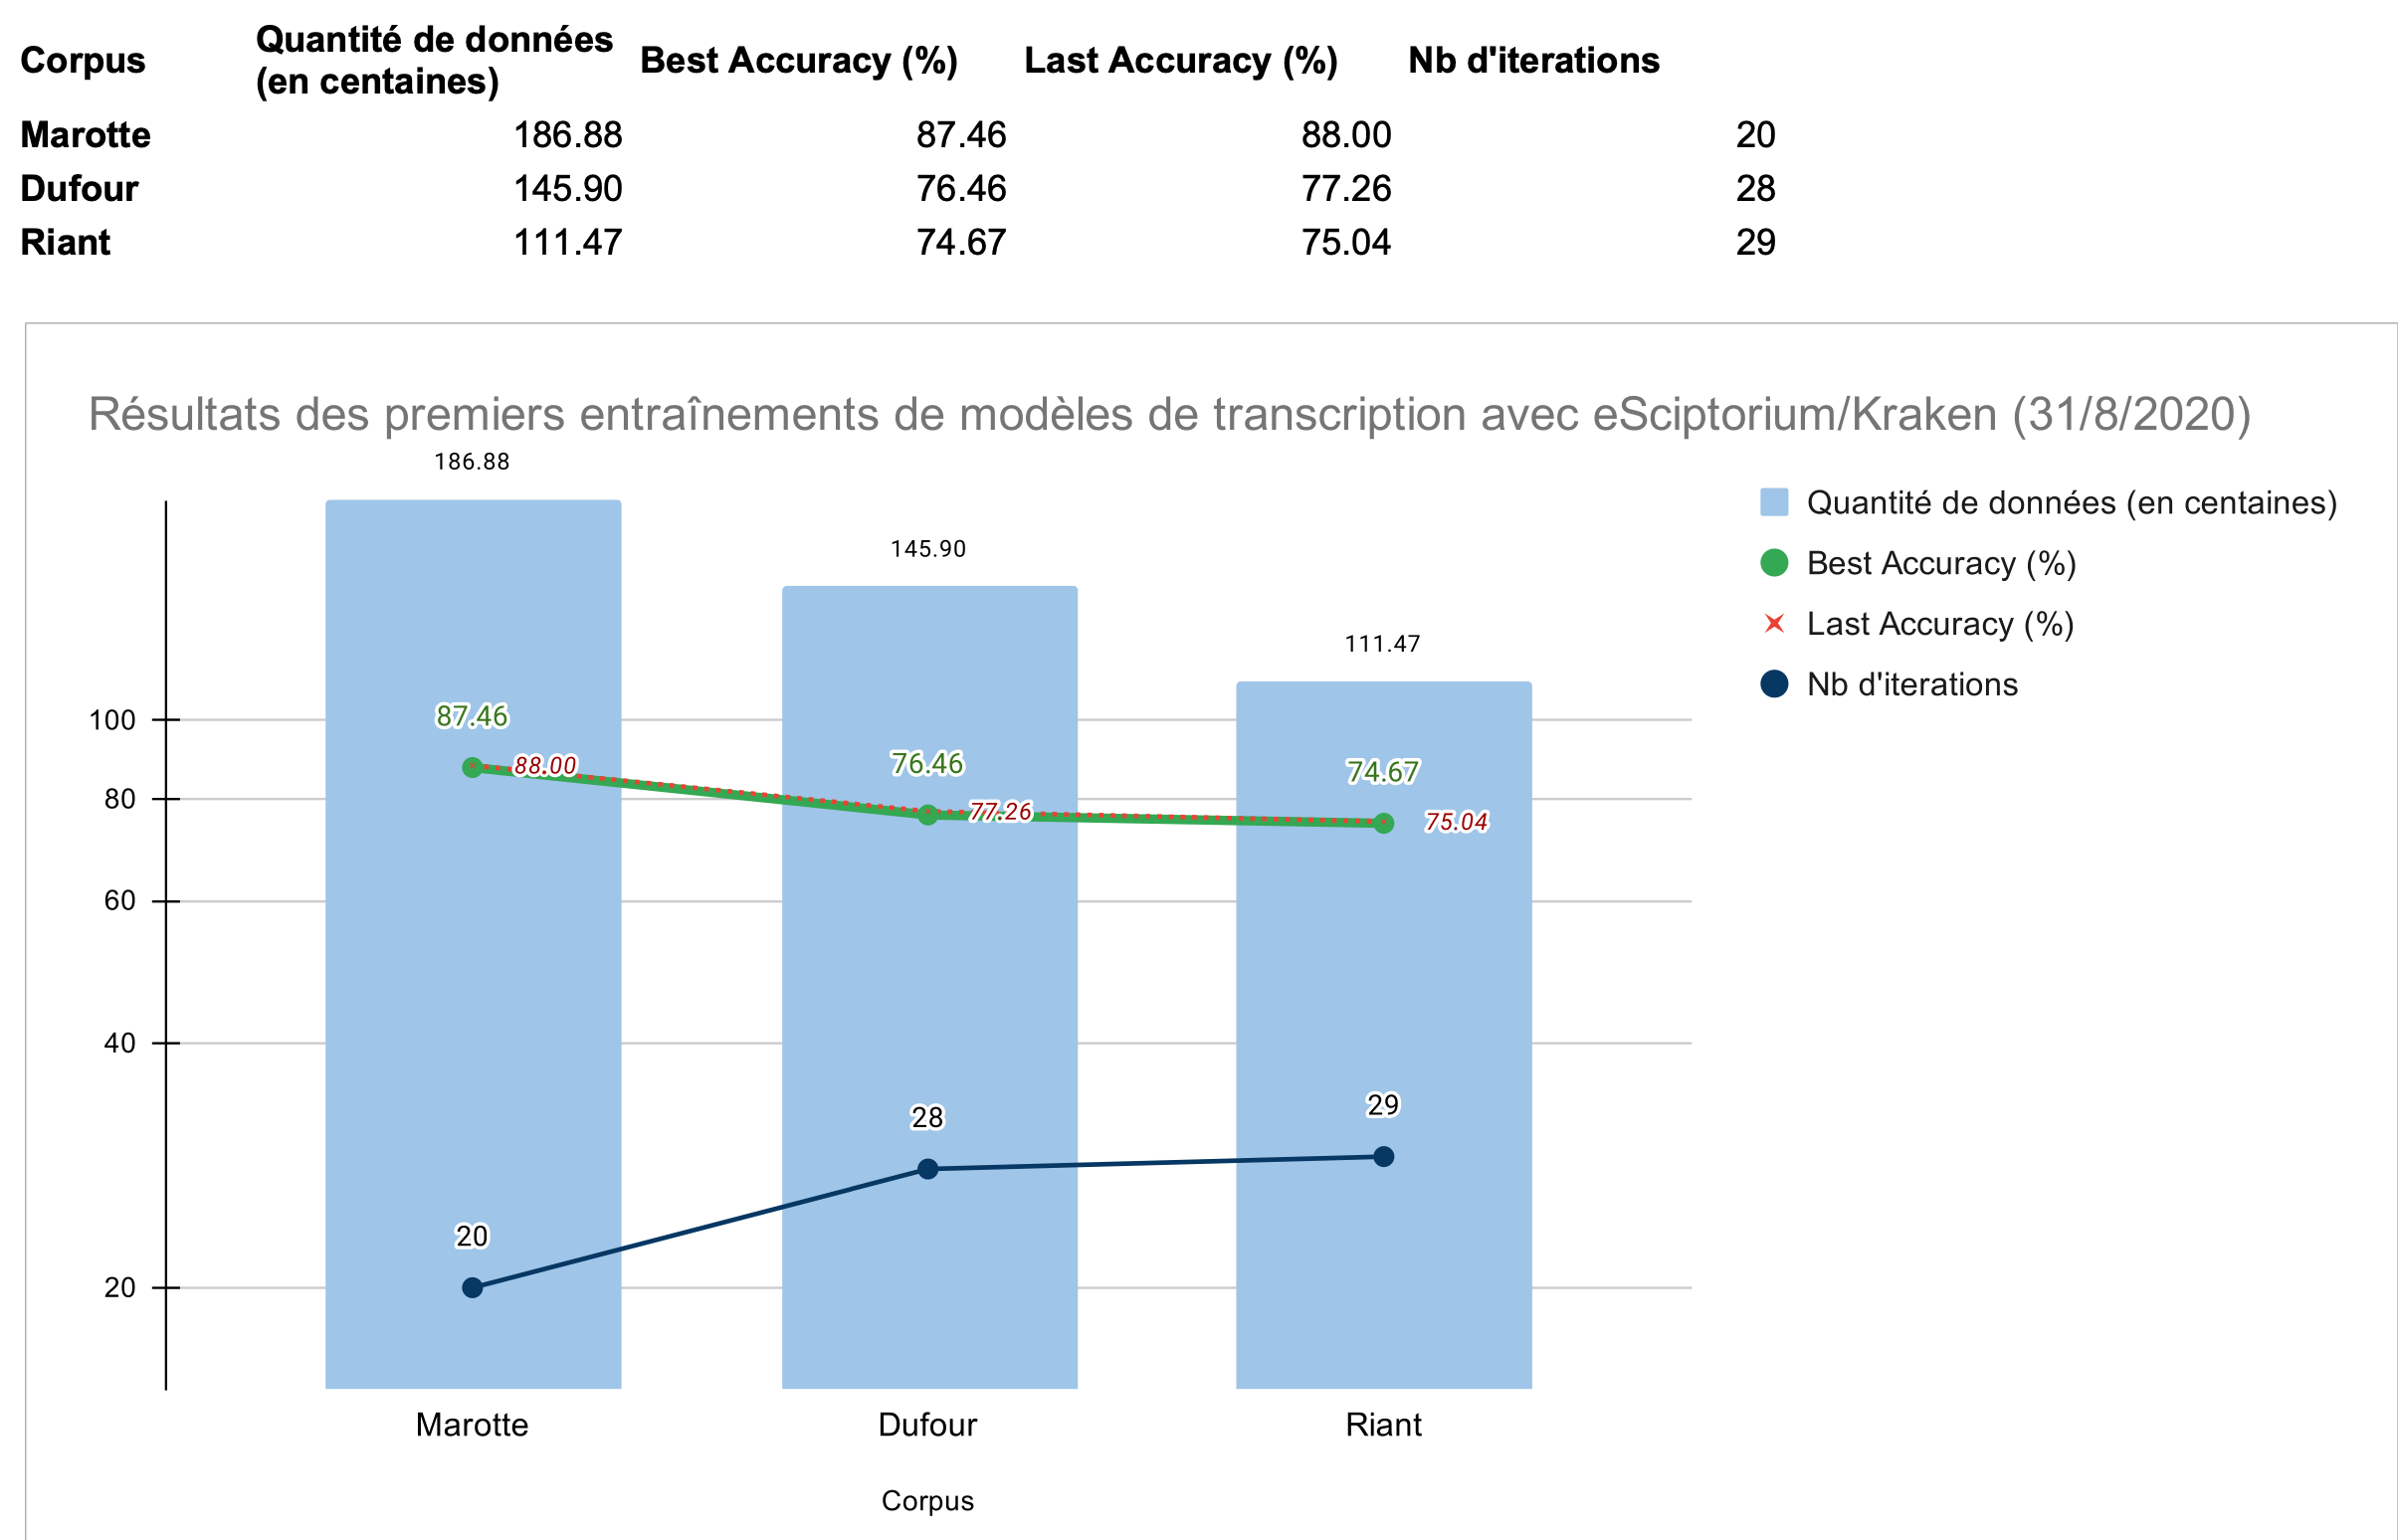
\includegraphics[width=15cm]{images_partie_3/eval_alix.png}}}
    \caption{Derniers entraînements de modèles réalisés pour Lectaurep   \textcopyright A. Chagué, 2020}
    \label{fig:visual_newmodels}
\end{figure}

Lectaurep gagnerait à entraîner un modèle sur des données plus nombreuses et hétérogènes. Sur ce dernier point, le \textit{Random set} sur l'espace \textit{ShareDocs}, initialement créé pour entraîner un modèle général de données mixtes, contient sept cents pages de notaires très différentes, qui pourrait être utilisé pour créer un modèle capable de s'appliquer à une plus grande diversité de mains, quitte à l'affiner pour des données plus spécifiques par la suite (\textit{Fine-tune}).\\

Cependant, l'ensemble des images de ce \textit{Random set} n'ont pas été encore était transcrites, et sont en cours d'annotation. La stratégie actuelle du DMC repose sur la transcription des images apparaissant dans l'ordre du \textit{Golden Set} - des lots de cent images homogènes (correspondant à un notaire)- afin de faciliter le travail des annotatrices et des annotateurs. Une approche compréhensible du point de vue du travail de transcription manuel, souvent fastidieux pour les annotatrices et les annotateurs, qui une fois avoir transcrit une ou deux pages de répertoire d'un notaire s'habituent rapidement aux écritures des autres images du même notaire; en effet, il peut être difficile pour une annotatrice ou un annotateur de sauter d'une écriture à l'autre. On remarque, que la réalité du travail d'annotation peut entrer en conflit avec la création d'un modèle de transcription général qui doit disposer de données variées pour traiter des cas nouveaux. On peut prévoir que cette méthodologie évoluera au sein du DMC dans la suite du projet afin d'obtenir de meilleurs résultats.


